\begin{refsection}[operations/hirakawa/group.bib]
%\nocite{*}
\chapter{HPCI System Development Team}

\section{Members}
\begin{itemize}
  \item[] Manabu Hirakawa (Team Leader)
  \item[] Etsuya Shibayama (Senior Visiting Scientist)
  \item[] Osamu Tatebe (Senior Visiting Scientist)
  \item[] Manabu Higashida (Visiting Scientist)
  \item[] Hiroshi Harada (Research \& Development Scientist)
%  \item[] Akira Kondo (Technical Staff)
%  \item[] Koichiro Ozaki (Technical Staff)
%  \item[] Chihiro Shibano (Technical Staff)
%  \item[] Hidetomo Kaneyama (Technical Staff)
%  \item[] Satomi Yasuda (Assistant)
\end{itemize}

\section{Research Activities}

We are involved in the technical development of an innovative high performance computing infrastructure (HPCI) that %
will connect the major Japanese supercomputers installed in universities and research institutes, including the %
K computer, through a network. The computing environment realized by HPCI will meet the diverse needs of its intended users. %
Furthermore, the high-speed network will enable the supercomputers, shared storage, and other functionalities of each HPCI %
system provider to operate as a common HPCI. To this end, we are working on the technical side of the system operation, %
the technical coordination of the facilities comprising HPCI system, and the operation of the HPCI Shared Storage (HPCI-SS).
 The HPCI-SS is a large-scale distributed file system comprising 4 meta-data and 40 file-data servers. The HPCI-SS forms %
the data-sharing infrastructure of the HPCI led by the Ministry of Education, Culture, Sports, Science and Technology. %
It provides a 22.5 PB single-view “Gfarm” network file system that is open to all HPCI users and supports scalable %
I/O performance in a geographically widely distributed environment. The HPCI-SS meta-data servers are located in RIKEN AICS %
and the University of Tokyo (U-Tokyo), while the file-data servers are located in AICS, U-Tokyo, %
and the Tokyo Institute of Technology (Tokyo Tech).%
 HPCI-SS also supports single sign-on authentication (GSI-AUTH), by which users can exchange their computational results between their %
local storage systems and HPCI-SS without additional authentication. %
HPCI-SS has developed into a key infrastructure for the management and sharing of computational data in HPCI projects.

% \begin{figure}
% \centering
%   \includegraphics[width=1.0\textwidth,keepaspectratio,natwidth=193,natheight=40]
%   {operations/hirakawa/fig/HPCI-SS-AR.png}
%   \caption{Overview of HPCI Shared Storage \& HPCI Archive}
%   \locallabel{fig:hpci-ssar}
% \end{figure}

\section{Research Results and Achievements}

%%%%%

\subsection{Technological Planning and Coordination}
For the Technological Planning and Coordination processes listed below, we offer total technical support across %
the entire HPCI system operation and coordination for other HPCI system providers that are in the same operating %
environment.

\begin{itemize}
  \item Oversee discussion tables for HPCI system providers.
  \item Conduct investigations and countermeasures for technical problems that arise in HPCI system operations.
  \item Review software improvements that are related to the entire HPCI system.
\end{itemize}

We maintain the HPCI system operation which needs to accommodate various requests from users %
of those services. In addition we work with the University of Tokyo, in the National University %
Corporation to maintain  the HPCI shared storage system. We provide data sharing storage for the community %
and computational resources for the pre-post processing of data.
\newline
As shown in Figure \localref{fig:hpci-overview}, the computational resources in the HPCI system are provided %
by the supercomputer centers of nine universities, RIKEN AICS and the Japan Agency for Marine-Earth %
Science and Technology (JAMSTEC). The Institute of Statistical Mathematics (ISM) has provided its %
resources since July 2014.

%\begin{figure}[htbp]
\begin{figure}[h]
 \begin{center}
  \begin{tabular}{c}

    \begin{minipage} {1.0\hsize}
     \begin{center}
      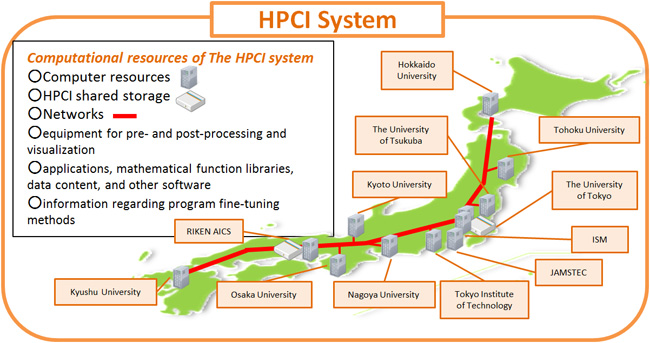
\includegraphics[clip, height=8cm] {./operations/hirakawa/fig/HPCI_System_en.jpg}
      \caption{Overview of the HPCI Structure.}
      \locallabel{fig:hpci-overview}
      \hspace{1.0cm}
     \end{center}
    \end{minipage}

   \end{tabular}
 \end{center}
\end{figure}

In FY2015, we coordinated and managed meetings for HPCI system providers and other relevant bodies.
\begin{itemize}
   \item We hosted three meetings of the HPCI Cooperation Service Committee.
   \item We hosted ten meetings of the HPCI Cooperation Service and Operation Working group.
   \item We hosted three meetings of the HPCI Shared Storage Operation team.
\end{itemize}

\subsection{HPCI System Monitoring}
HPCI system monitoring allows us to monitor the status of the computing resources provided %
by each HPCI system provider, the operational status of the network, and the bandwidth and %
throughput performance. The HPCI system monitoring has the following duties:
\begin{itemize}
  \item To investigate the causes of and response measures to technical problems that occur during the operation of the HPCI system.
  \item To research improvements in software related to the operation of the overall HPCI system.
  \item To operate and maintain the HPCI shared storage site (the West site);
  \item To operate and maintain the management of the Login Gateway and the HPCI IdP of AICS (one of the HPCI system provider);
  \item To develop the HPCI online application system;
  \item To screen institutions seeking to participate in the shared operation (i.e., seeking to provide computing resources to the HPCI system) to check whether they satisfy the technical requirements.
\end{itemize}

\begin{figure}[h]
 \begin{center}
  \begin{tabular}{c}

    \begin{minipage} {1.0\hsize}
     \begin{center}
      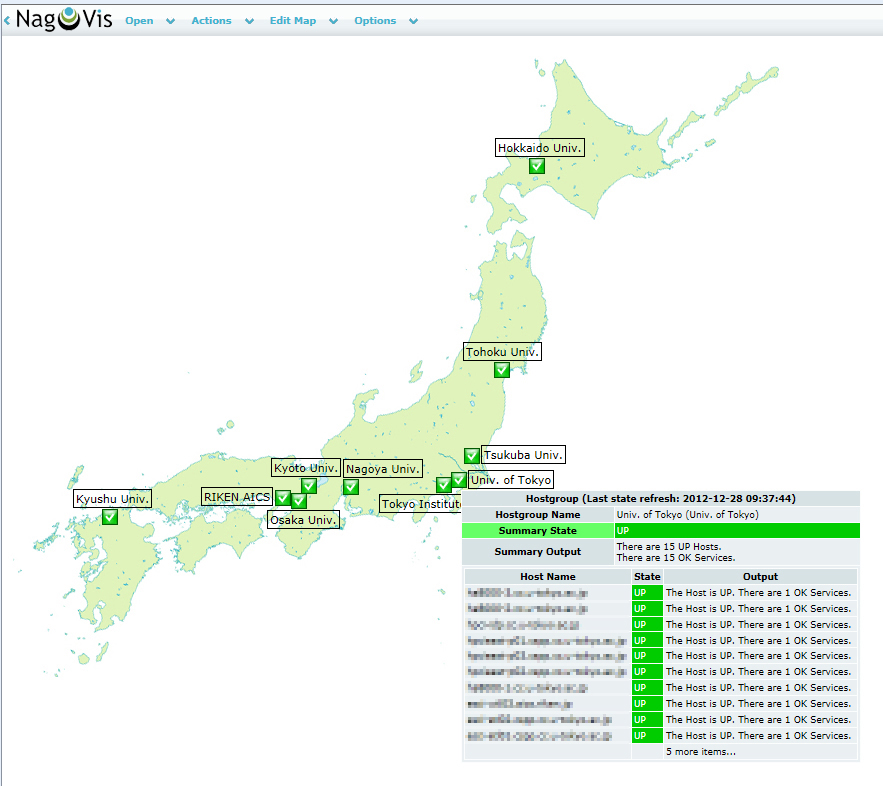
\includegraphics[clip, height=10cm] {./operations/hirakawa/fig/Nagios.jpg}
      \caption{The overall Nagios/Nagvis monitoring system.}
      \locallabel{fig:nagios}
     \end{center}
    \end{minipage}

   \end{tabular}
 \end{center}
\end{figure}

%%%%%%%%%%%%%%%%%%%%

\subsection{HPCI Shared Storage System}

\begin{figure}[h]
\centering
  \includegraphics[width=1.0\textwidth,keepaspectratio,natwidth=193,natheight=40]
%  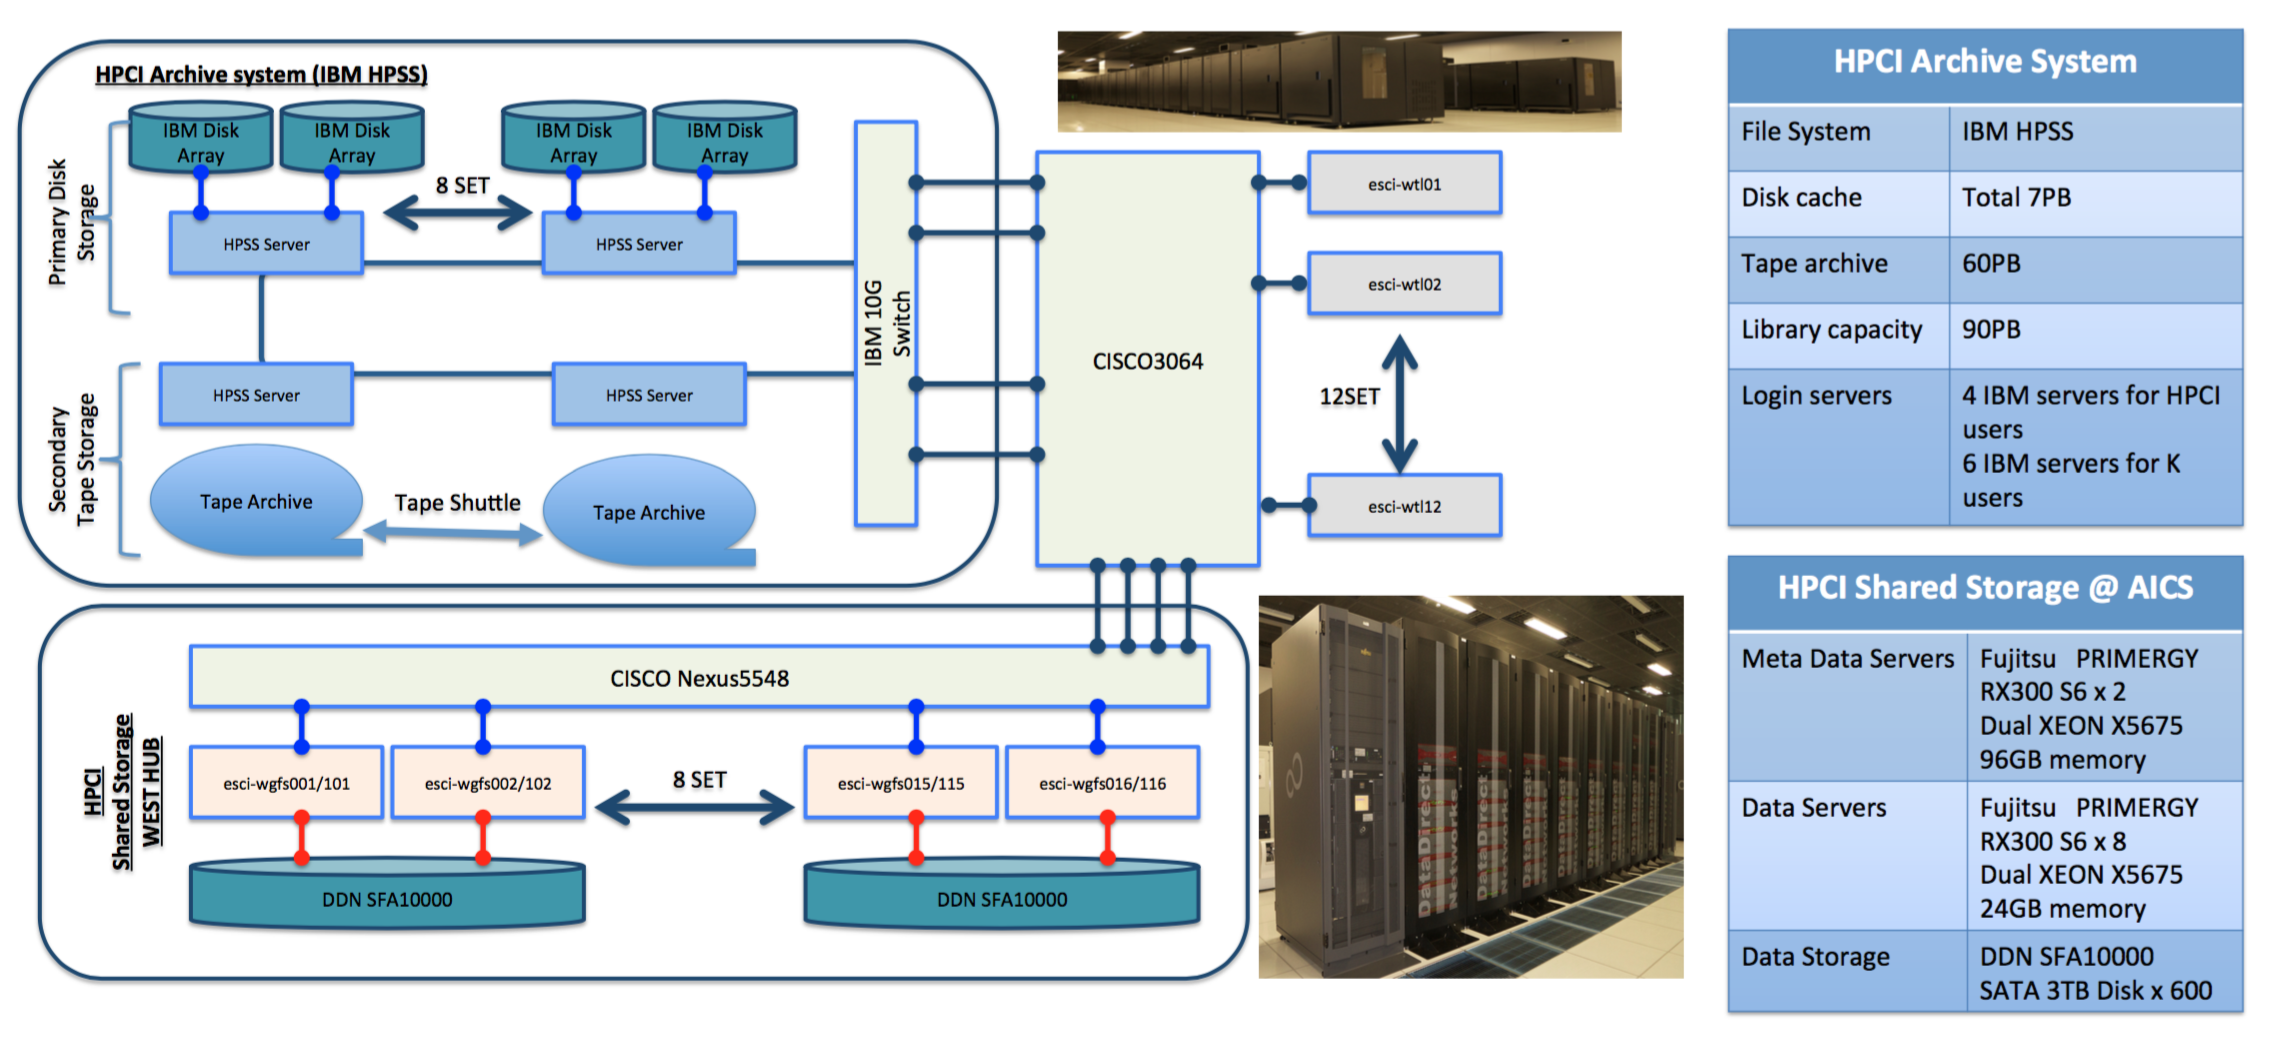
\includegraphics[clip, height=5cm,keepaspectratio]
  {operations/hirakawa/fig/HPCI-SS-AR.png}
  \caption{An overview of the HPCI Shared Storage and HPCI Archive Systems.}
  \locallabel{fig:hpci-ssar}
\end{figure}

In FY2015, HPCI-SS was used by 70 HPCI projects and the total requested storage size was nearly two times the physical storage size %
% \cite{Gfarm-WS-2015}.
To cope with this demand, we determined a new resource allocation policy as follows.
\begin{itemize}
  \item The maximum size of each project is set to 1.6 PB.
  \item The average number of file replicas is set to 1.5 (compared to 2 in FY2014).
\end{itemize}

Figure \localref{fig:ss-diskusage} shows the HPCI-SS disk usage from FY2014 to FY2015.  As shown in these graphs, even though the %
HPCI-SS file usage is increasing, the disk usage is decreasing. This is the result of the new allocation policy.

%%%%%%%%%%%%%
%%%%%%%%%%%%%
%
%  http://qiita.com/poemn/items/9142339749c87ebdb536
%
%  図を並べて配置
% http://www.latex-cmd.com/fig_tab/alignment.html
%
%

%\begin{figure}[h]
\begin{figure}
 \begin{center}
  \begin{tabular}{c c}

    \begin{minipage} {0.5\hsize}
     \begin{center}
      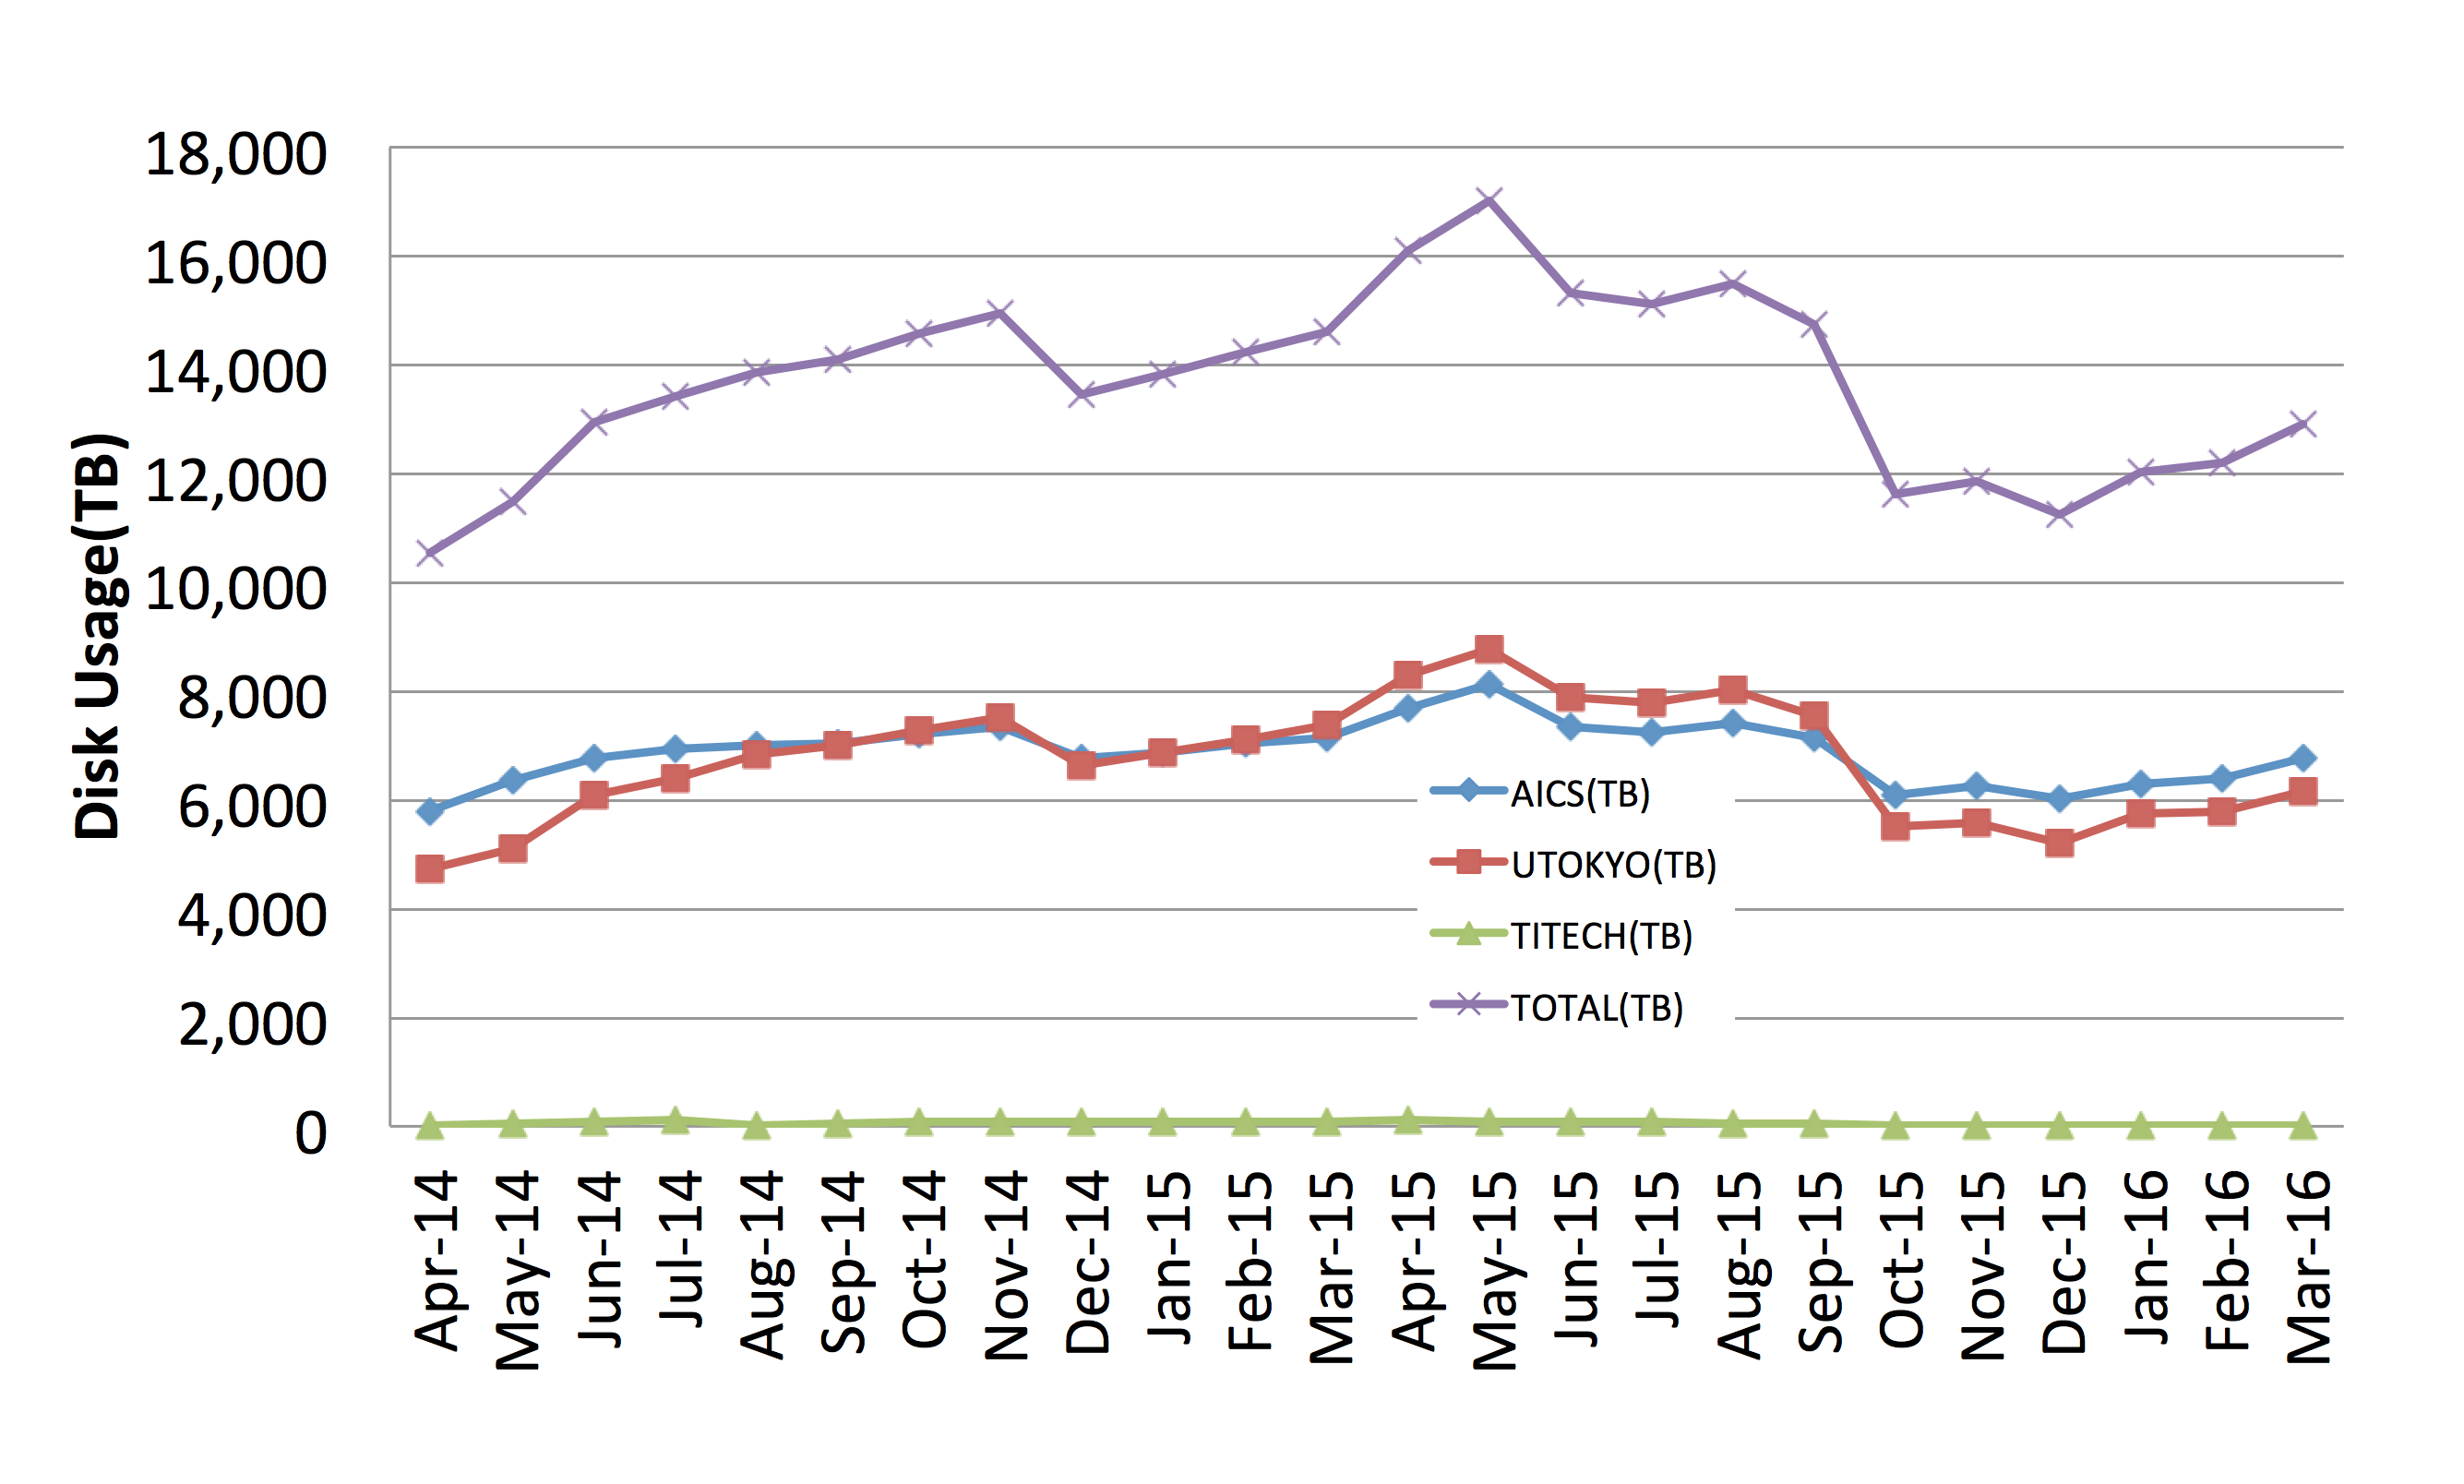
\includegraphics[clip, height=6cm, width=7cm] {./operations/hirakawa/fig/SS-DiskUsage.png}
      \caption{HPCI Shared Storage disk usage.}
      \locallabel{fig:ss-diskusage}
      \hspace{1.6cm}
     \end{center}
    \end{minipage}

    \begin{minipage} {0.5\hsize}
     \begin{center}
      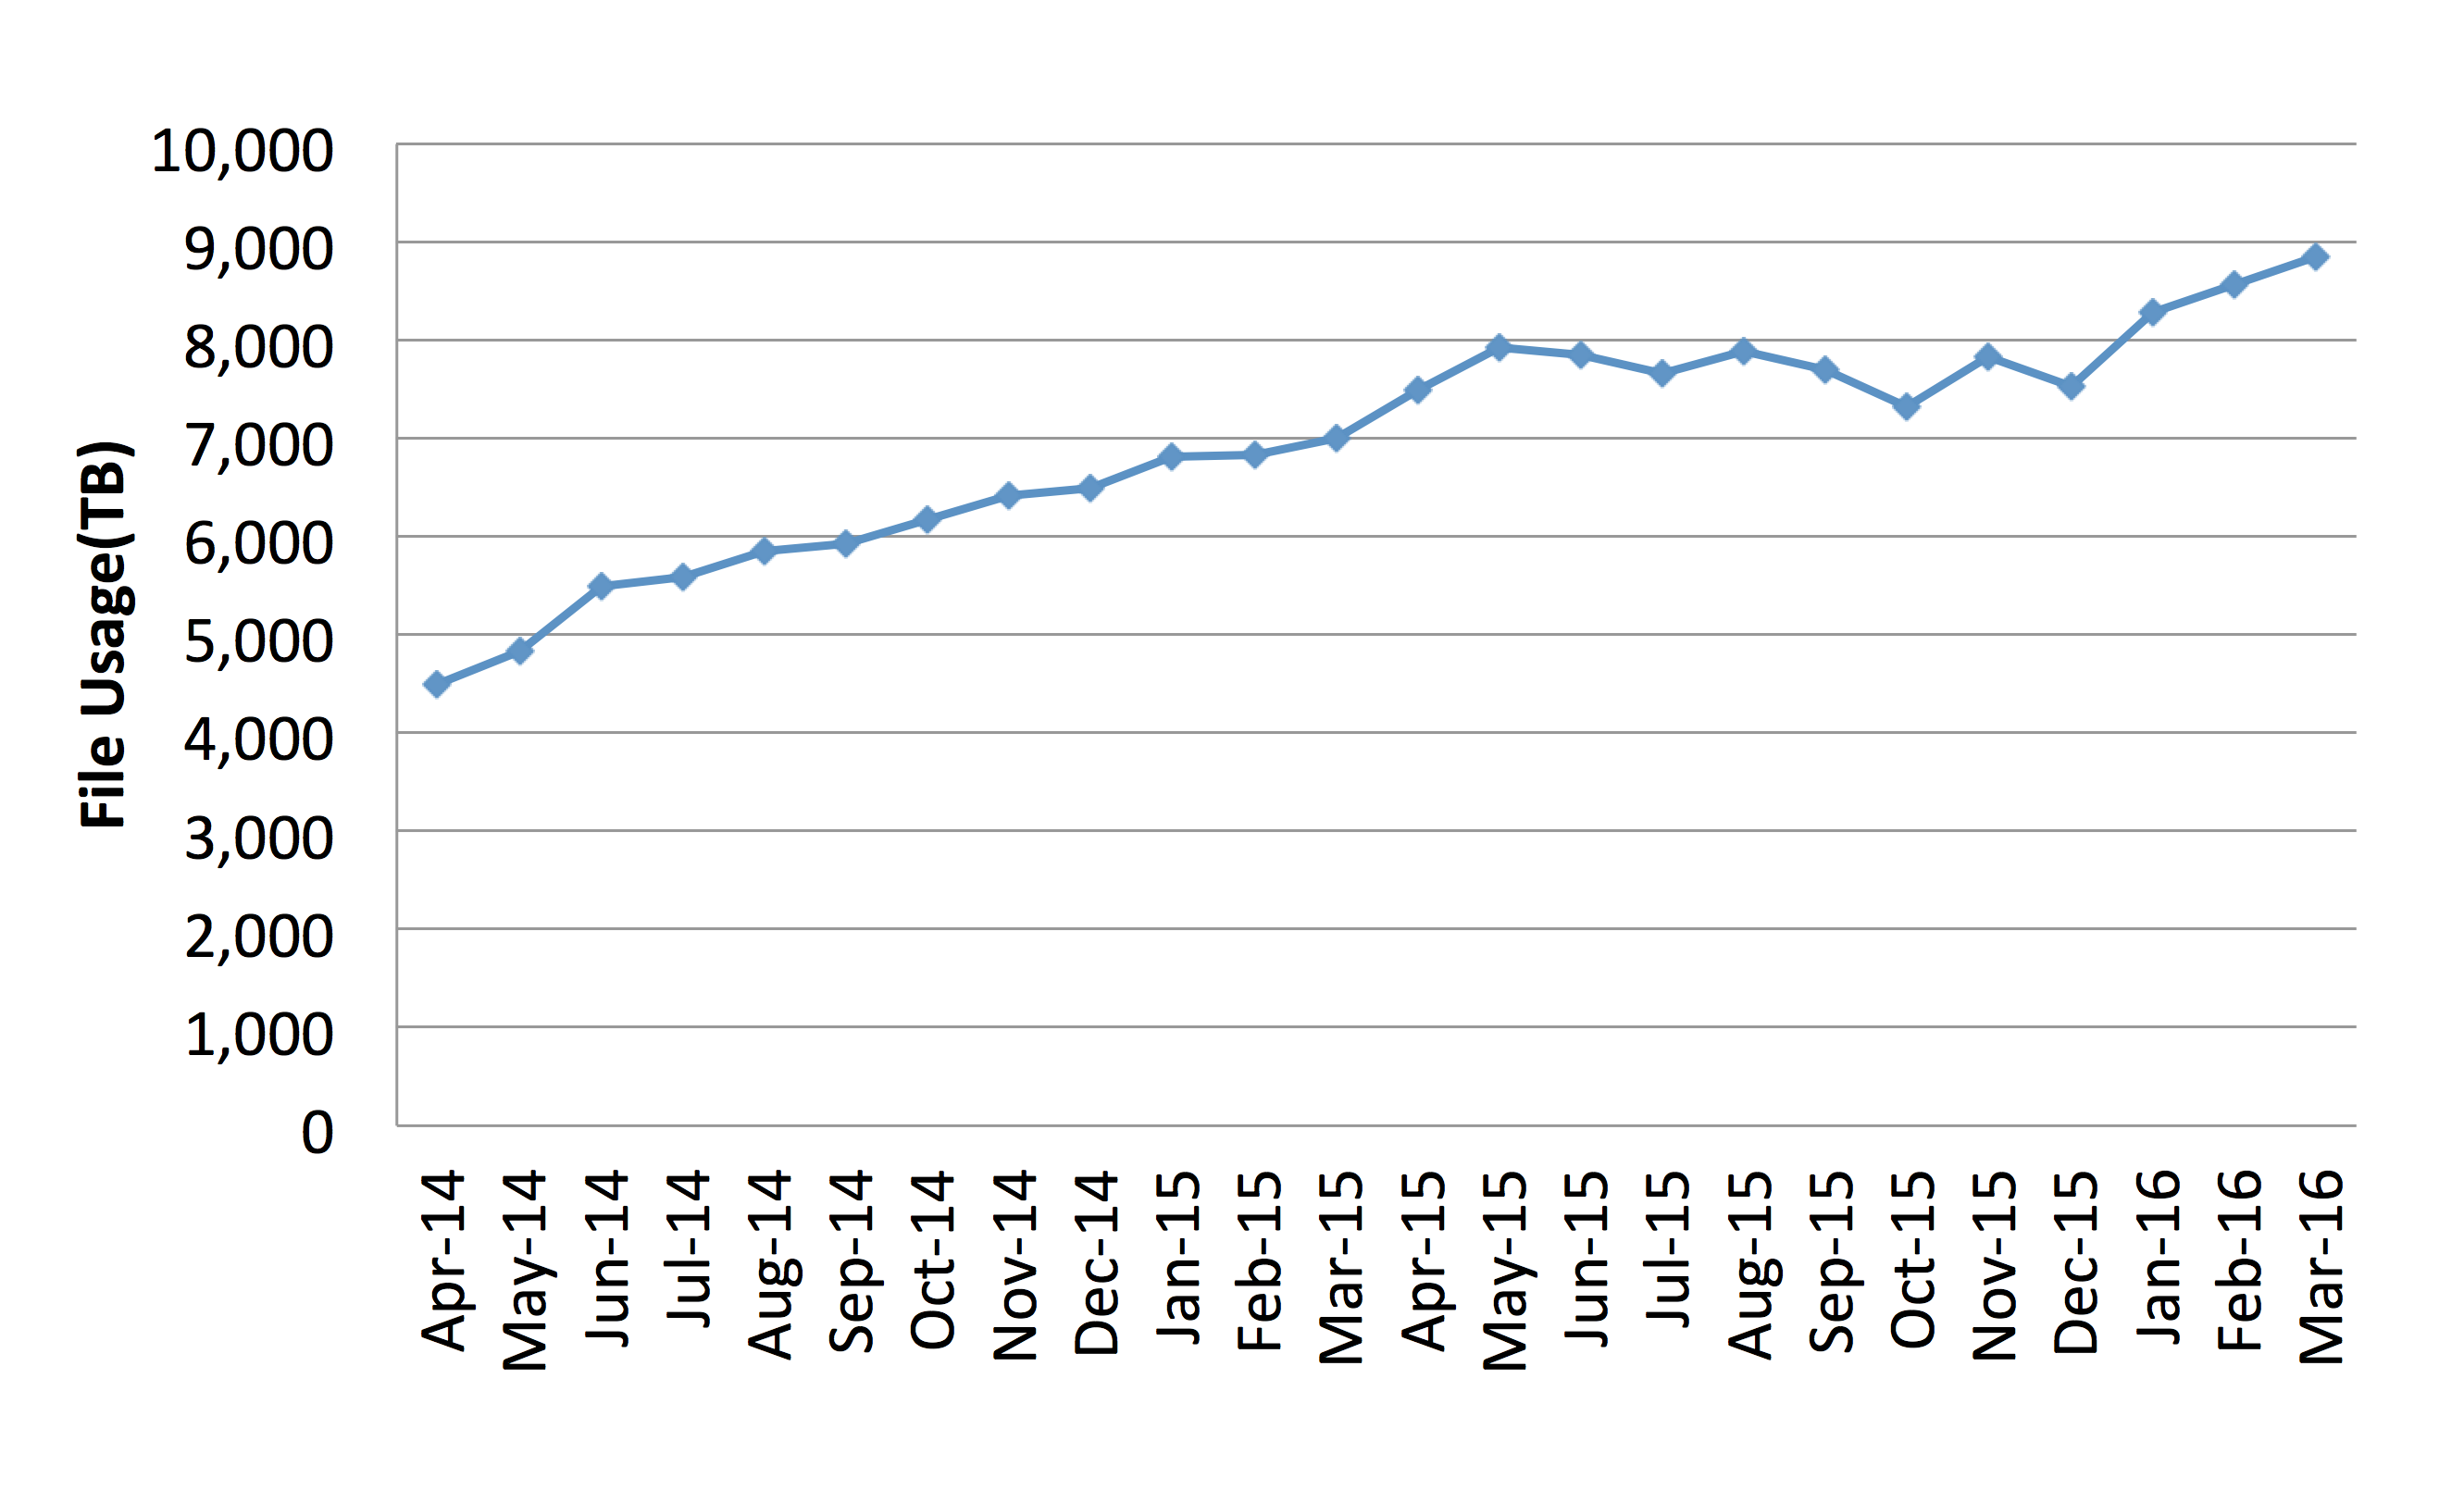
\includegraphics[clip, height=6cm, width=7cm] {./operations/hirakawa/fig/SS-FileUsage.png}
      \caption{HPCI Shared Storage file usage.}
      \locallabel{fig:ss-fileusage}
      \hspace{1.6cm}
     \end{center}
    \end{minipage}
   \end{tabular}
  \end{center}
 \end{figure}

%%%%%%%%%%

\subsubsection{Periodic Data Integrity Check for Data Corruption}
HPCI-SS with its Gfarm file system supports data integrity checks. %
A file digest is calculated at the storage node before the data is written to storage and is stored in metadata.%
A file digest is also calculated when reading the entire data in a file. %
Data corruption can be detected by comparing the metadata digest to the file data digest via the gfspooldigest command. %
At the AICS site, data integrity checks are done on a weekly basis.  %
All the created and updated files' data integrity checks can be completed within a week. %
The results of the periodic data integrity checks are managed on the HPCI web page.
%\cite{Gfarm-Symp-2015}\cite{AXIES-HARADA-2015}.

\begin{figure}[h]
\centering
  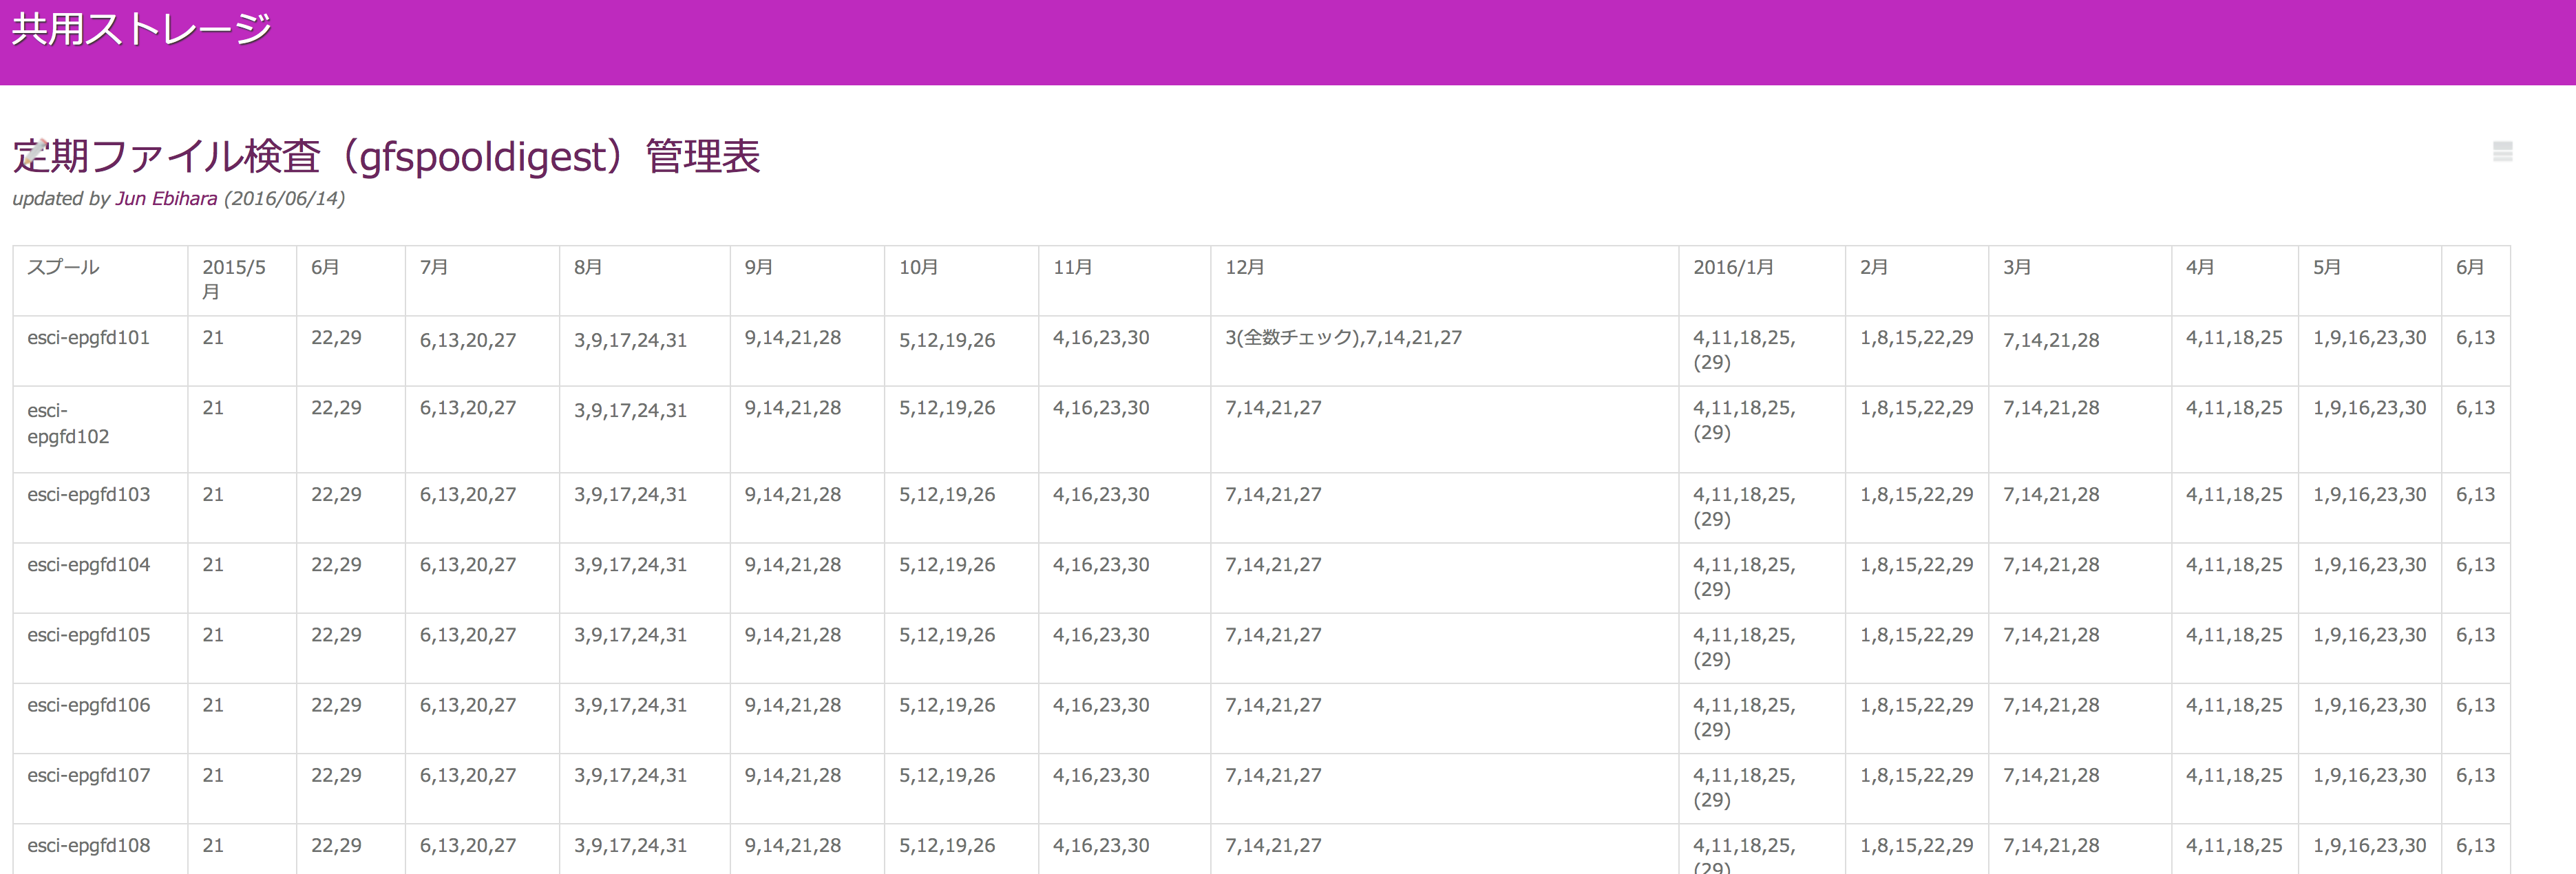
\includegraphics[width=1.0\textwidth,keepaspectratio,natwidth=193,natheight=40]
  {operations/hirakawa/fig/DataIntegrityCheck.png}
  \caption{History of the data integrity checks.}
  \locallabel{fig:DataIntegrityCheck}
\end{figure}

%% To cope with data corruption, \\
%% And the read system call returns input/output error when the digest mismatches.

\subsubsection{Operational guidelines based on ITIL}
To improve the standard level of our HPCI-SS system operations, we dicided to introduce the ITIL methodology. %
% \cite{AXIES-NAKA-2015}.
First, we analyzed our operations using the ITIL methodology, and many improvements were made. %
Then we examined the service level, the quality of operation, and our relationships with our partners. %
Finally, a new HPCI-SS operational guideline was established. To satisfy our operational guideline, we evaluated our members' skills, %
documentations, personnel distributions, and management roles, in addition to multiple other points.

\begin{figure}[h]
\centering
  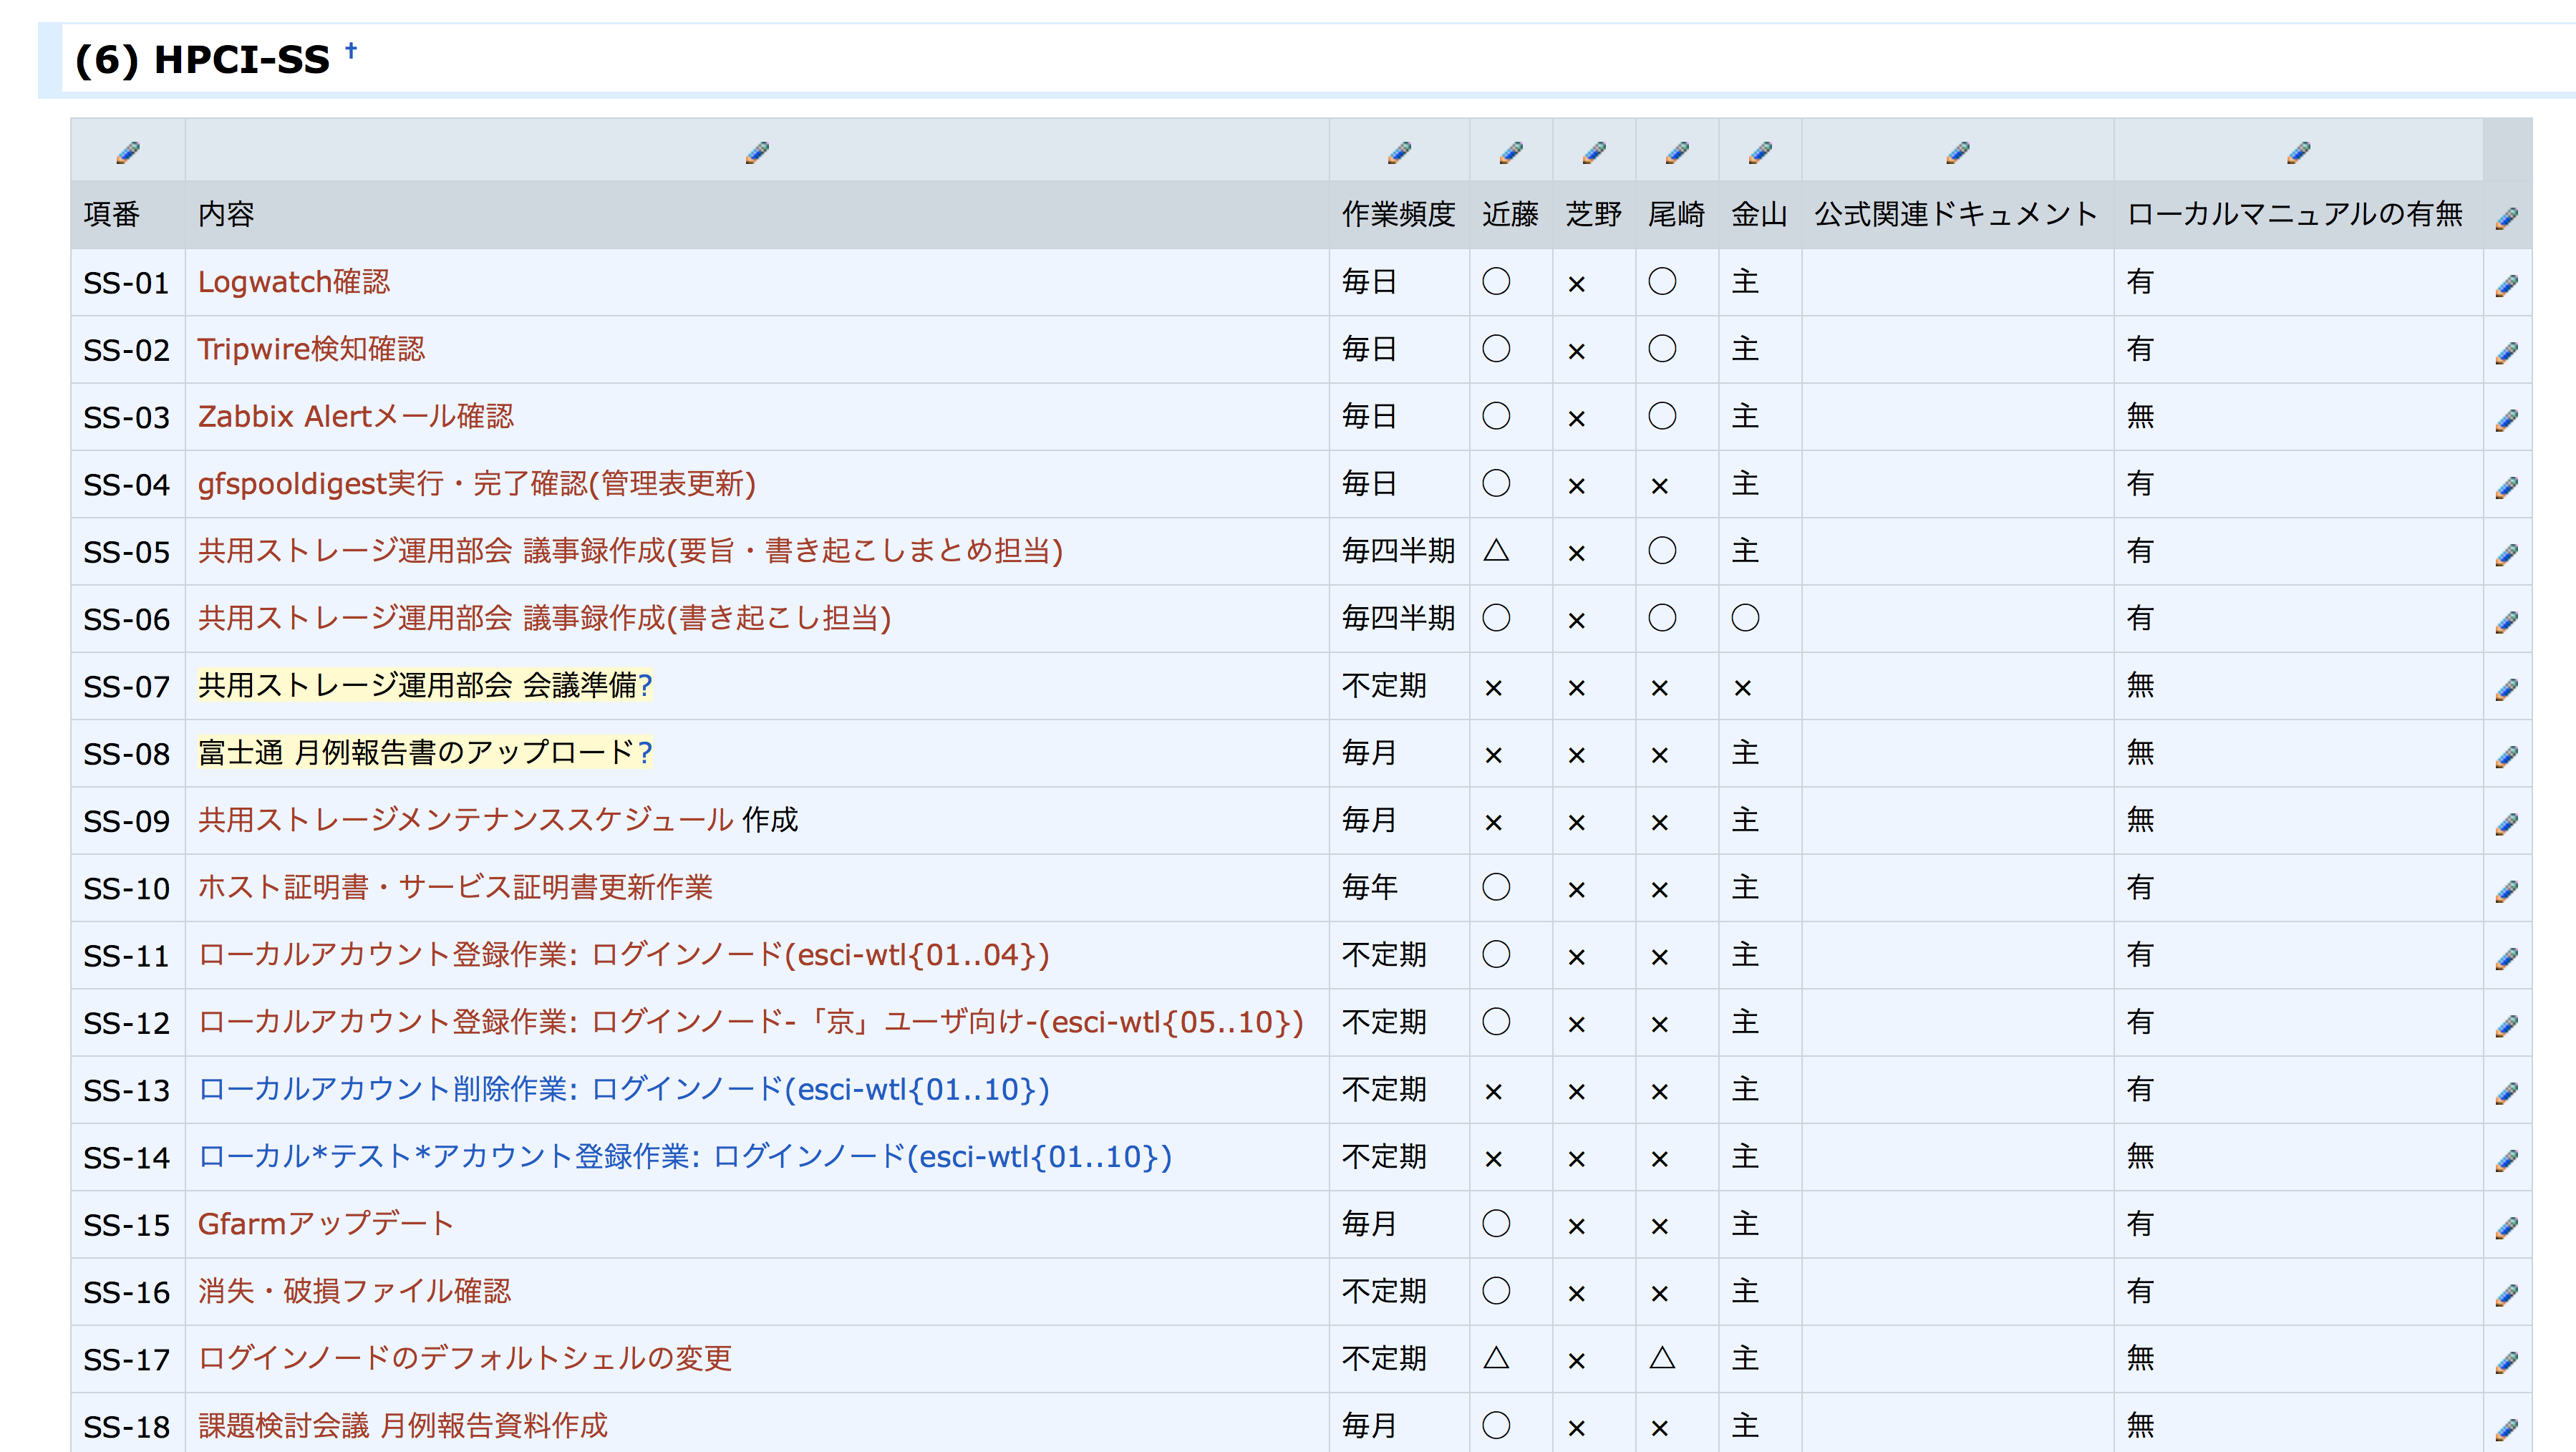
\includegraphics[width=1.0\textwidth,keepaspectratio,natwidth=193,natheight=40]
  {operations/hirakawa/fig/SkillMap.png}
  \caption{The HPCI-SS skill map.}
  \locallabel{fig:SkillMap}
\end{figure}

\subsection{User Support}
In collaboration with the U-Tokyo and Tokyo Tech teams, the HPCI System Development Team has developed additional %
user support system, such as HPCI user management and Gfarm consulting services.
\begin{itemize}
  \item 700 or more scientists were using HPCI-SS by the end of FY2015. User support is provided through the HPCI Help desk and the hpci-tech@aics.riken.jp mailing list.
  \item Technical information concerning HPCI-SS and HPCI-AS, including the system configuration, manuals, tips, services, and maintenance schedules, are available through the HPCI CMS website, Figure \localref{fig:UserSupport}.
  \item The HPCI-SS usage for each project is conveyed to project leaders in our monthly reports.
  \item Technical consulting services on HPCI-SS are provided by Prof. Tatebe, U-Tokyo, and Tokyo-Tech.
\end{itemize}

\begin{figure}[h]
\centering
  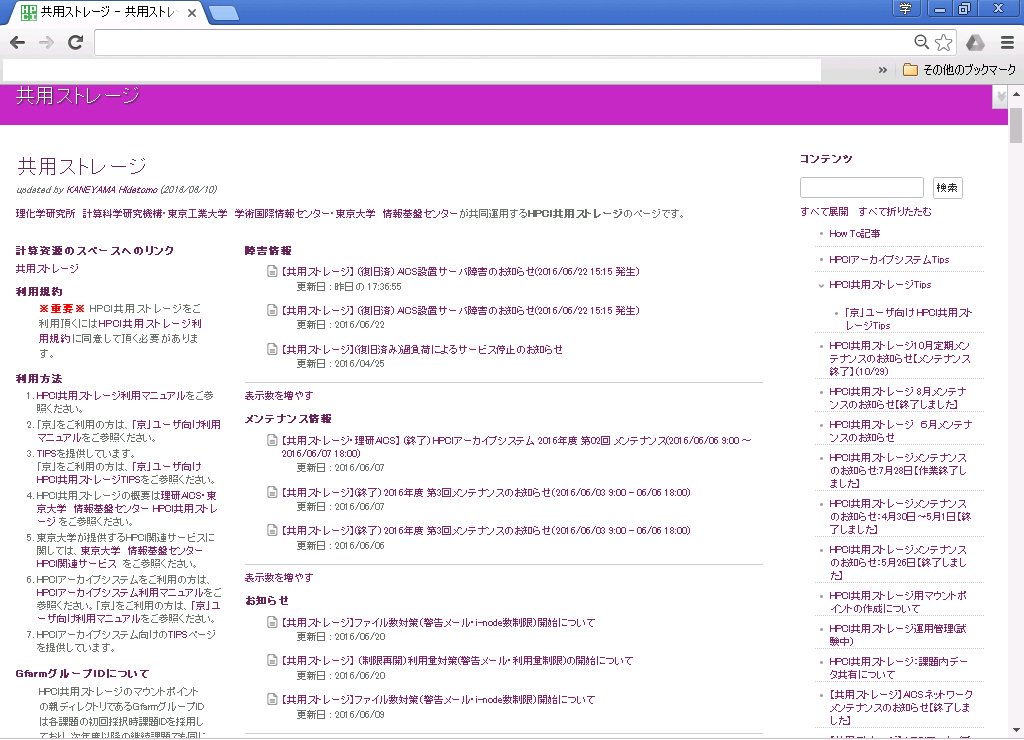
\includegraphics[width=1.0\textwidth,keepaspectratio,natwidth=193,natheight=40]
  {operations/hirakawa/fig/HPCI-SS-UserSupportPage.jpg}
  \caption{An HPCI-SS user support page.}
  \locallabel{fig:UserSupport}
\end{figure}


% \subsection{Long-term data archive project}
\subsection{HPCI Archive System for long-term  data archives}
By the end of  FY2015, a total of 4.4 PB of computational data from 43 HPCI %
research projects was archived in the HPCI Archive system. %
In addition, the computational data of 8 expired research projects were archived to comply with %
a Research Organization for Information Science and Technology (RIST) request.

Figures \localref{fig:ar-usage} \_ \localref{fig:ar-avgsize} show the total usage, file-counts, %
and average-size of the HPCI Archive system. %
In addition, Figures \localref{fig:ar-SizeDistribution} and \localref{fig:ar-CountDistribution} illustrate %
the file counts and size distributions on the HPCI Archive System.

As shown in the graphs, the total usage and file counts are increasing, %
and the average file size is decreasing. %
Large numbers of small files can cause performance degradation. %
Therefore, the average file size must be carefully monitored. %
Currently, the number of files smaller than 100 MB occupy 9.89 \% of the archive.

% The Research Organization for Information Science and Technology (RIST) requested that the computational data of expired %
% research projects be archived in HPCI-AS for three years. Complying with this request, 119 TB of the computational data of five %
% expired projects were archived in FY2015 and will be saved until the end of FY2018.

%%%%%%%%%%%%%%%%%% HPCI Archive Stats%%%%%%%%%%%%%%%%%%%%%%%%
\begin{figure}[h]
 \begin{center}
  \begin{tabular}{c}

    \begin{minipage} {0.33\hsize}
     \begin{center}
      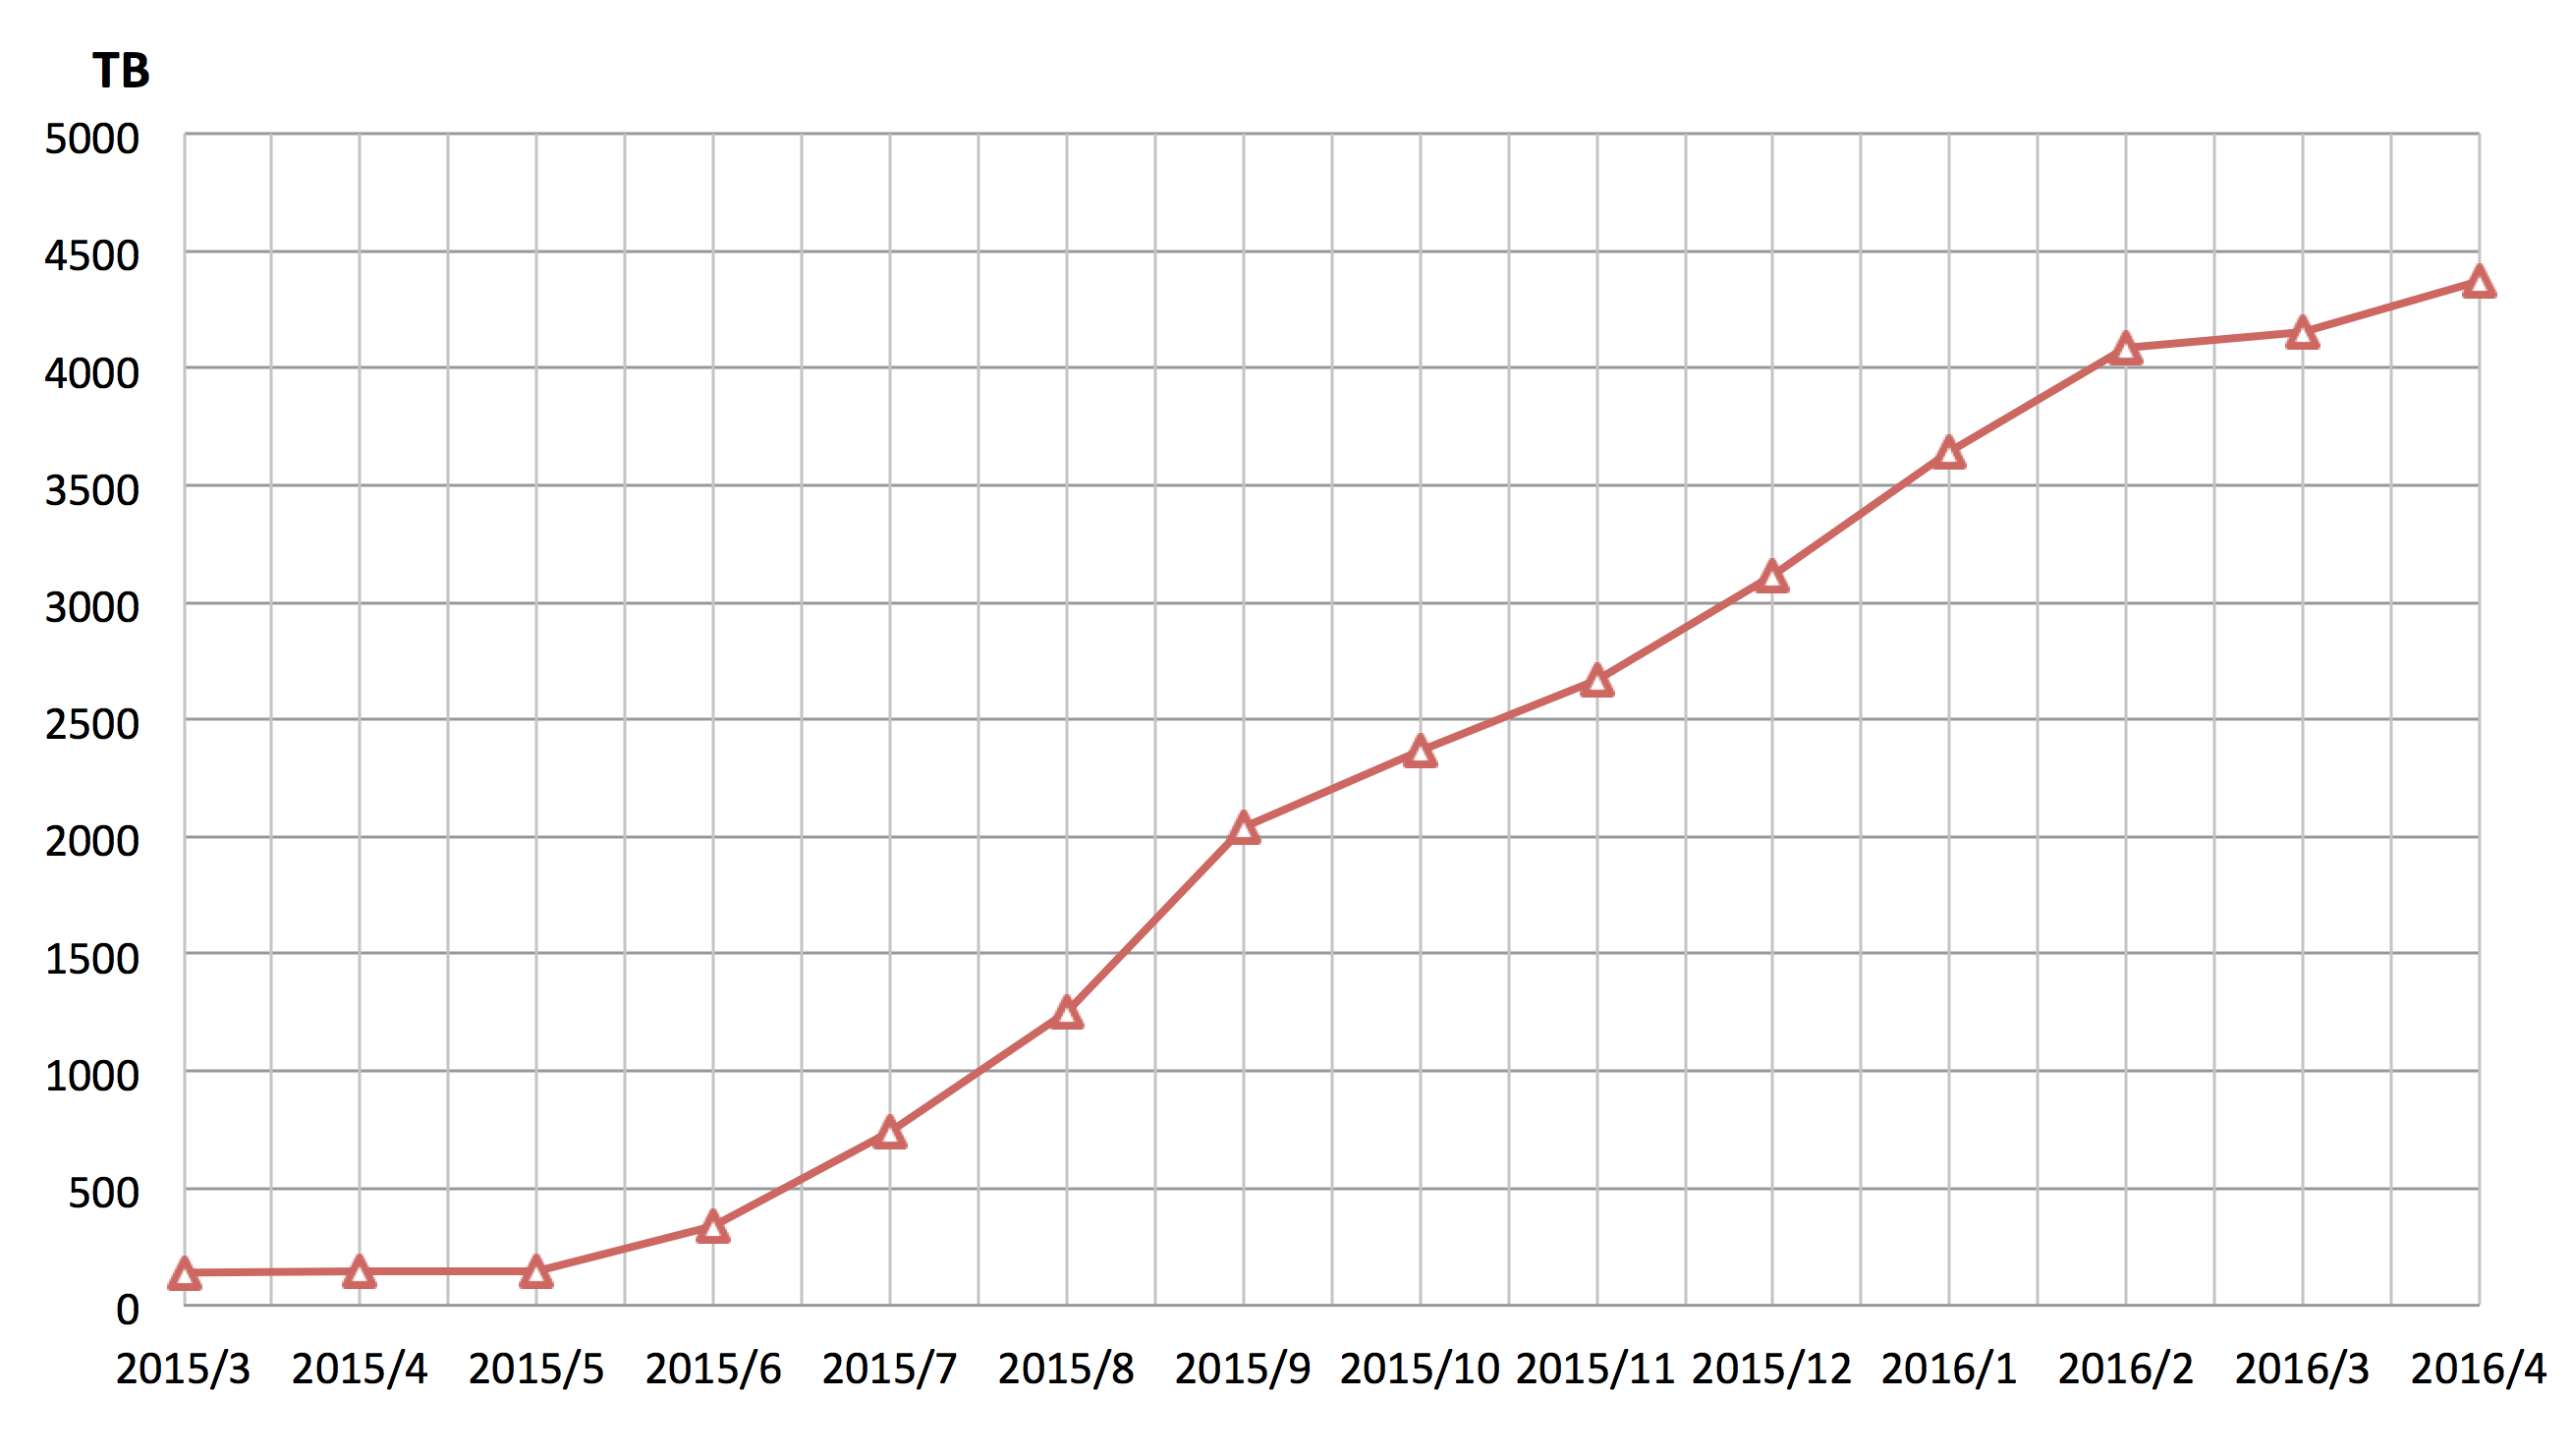
\includegraphics[clip,height=5cm, width=5cm]  {operations/hirakawa/fig/ArchiveUsage.png}
      \caption{Usage of the HPCI Archive System.}
      \locallabel{fig:ar-usage}
%      \hspace{1cm}
     \end{center}
    \end{minipage}

    \hspace{0.4cm}

     \begin{minipage} {0.33\hsize}
     \begin{center}
     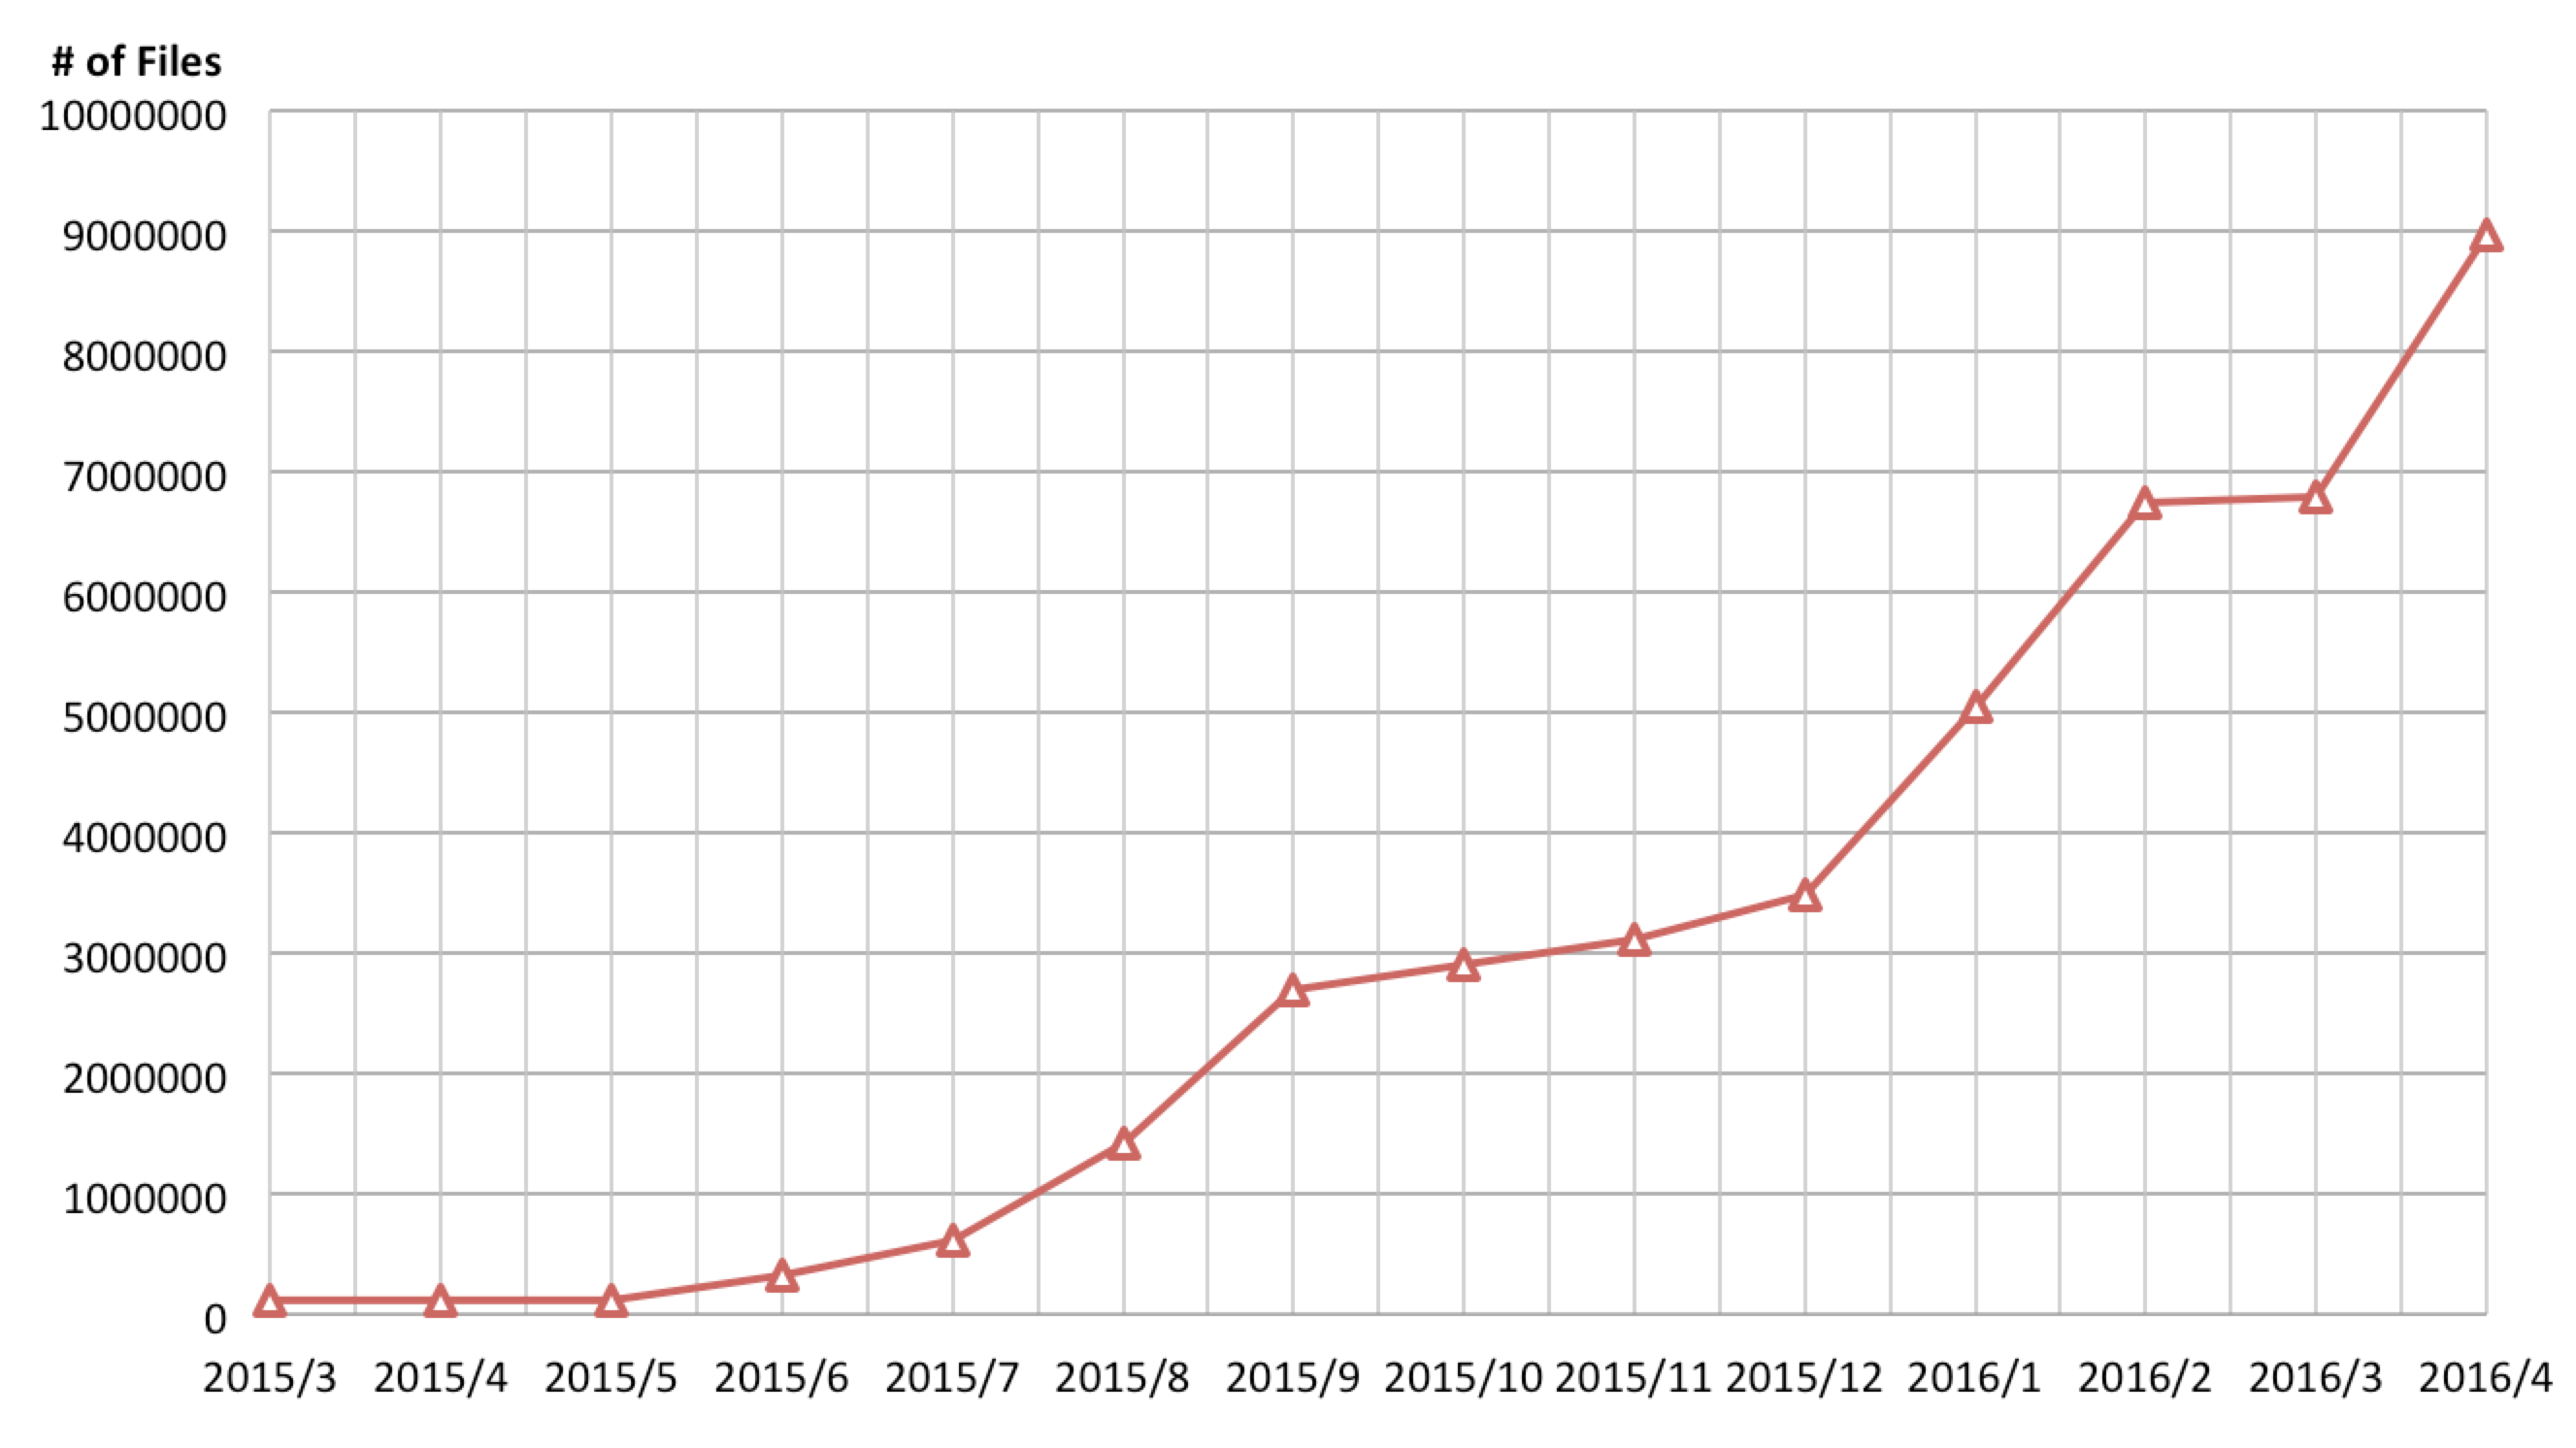
\includegraphics[clip, height=5cm, width=5cm]  {operations/hirakawa/fig/ArchiveFileNum.png}
      \caption{Number of HPCI Archive System files.}
      \locallabel{fig:ar-counts}
%      \hspace{1cm}
     \end{center}
    \end{minipage}

   \hspace{0.4cm}

    \begin{minipage} {0.33\hsize}
     \begin{center}
      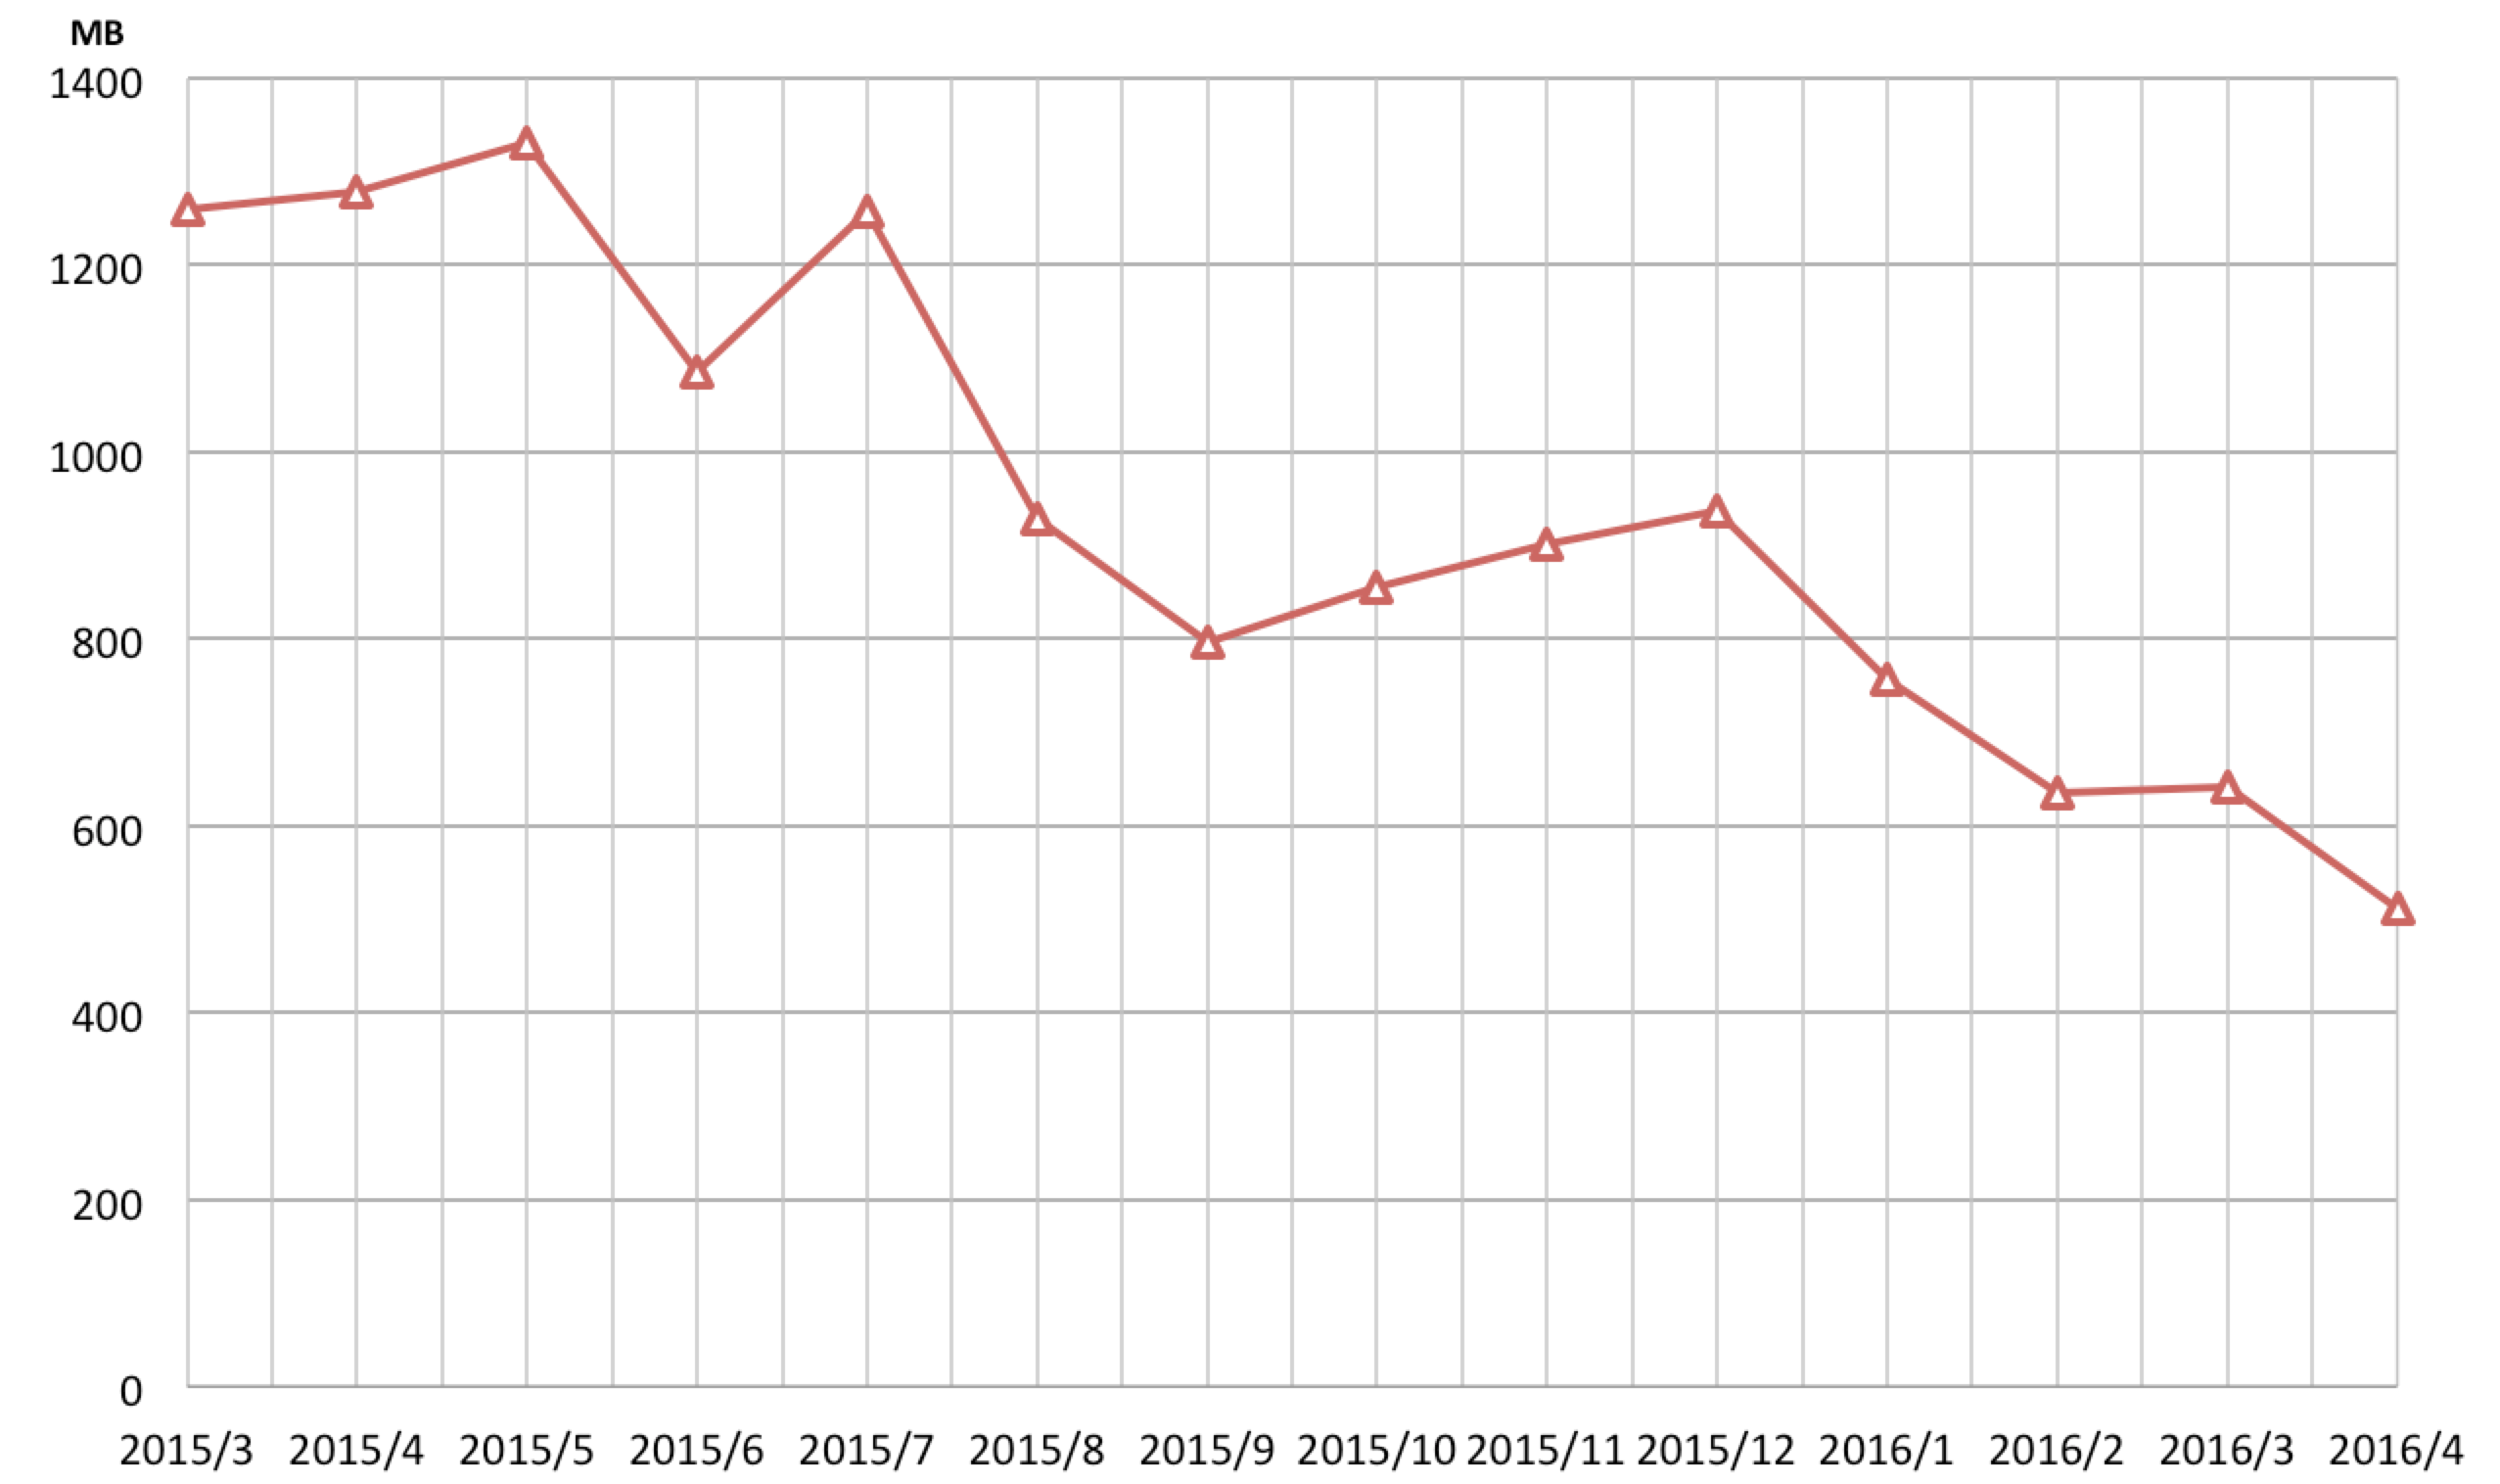
\includegraphics[clip, height=5cm, width=5cm]  {operations/hirakawa/fig/ArchiveAvgSize.png}
      \caption{Average file size in the HPCI Archive System.}
      \locallabel{fig:ar-avgsize}
%      \hspace{1cm}
     \end{center}
    \end{minipage}

  \end{tabular}
 \end{center}
\end{figure}

%%%%%%%%%%%%%%%%%% Distribution Map %%%%%%%%%%%%%%%%%%%%%%%%
\begin{figure}[h]
 \begin{center}
  \begin{tabular}{c}

    \begin{minipage} {0.5\hsize}
     \begin{center}
      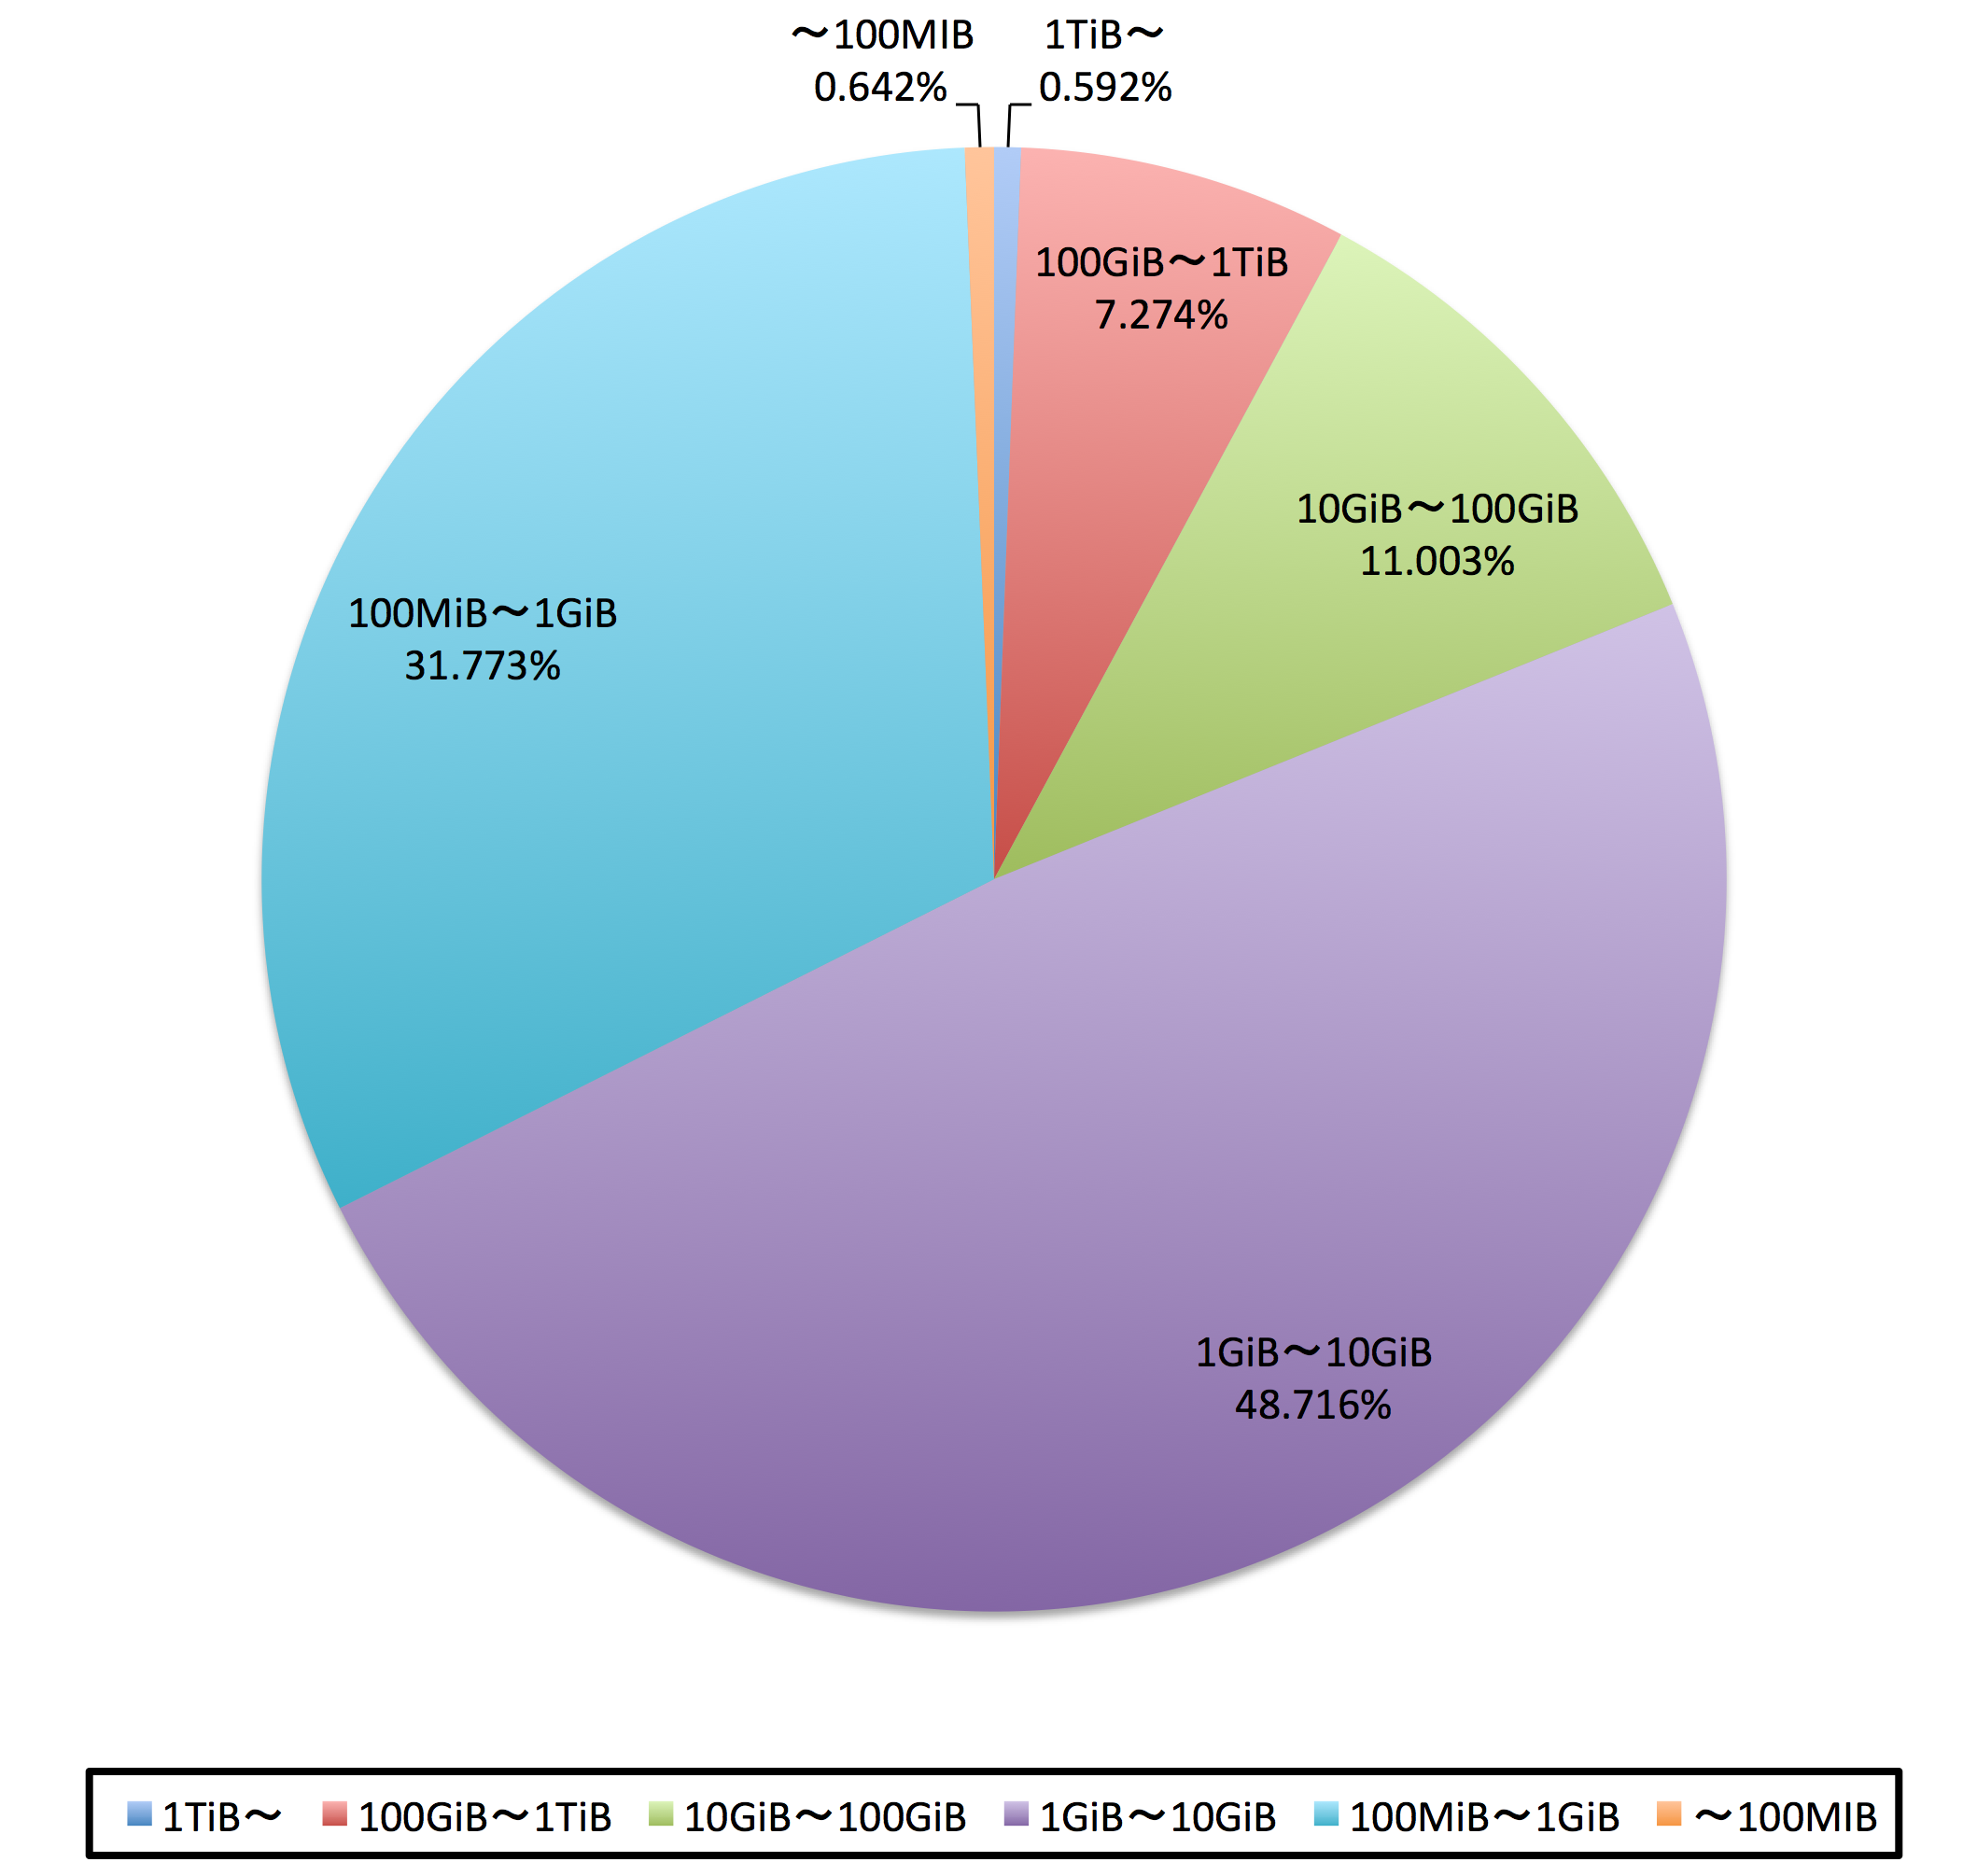
\includegraphics[clip, height=7cm, keepaspectratio] {operations/hirakawa/fig/ArchiveFileSizeDistribution.png}
      \caption{File size distribution in the HPCI Archive System.}
      \locallabel{fig:ar-SizeDistribution}
      \hspace{1cm}
     \end{center}
    \end{minipage}

    \hspace{0.6cm}

    \begin{minipage} {0.5\hsize}
     \begin{center}
      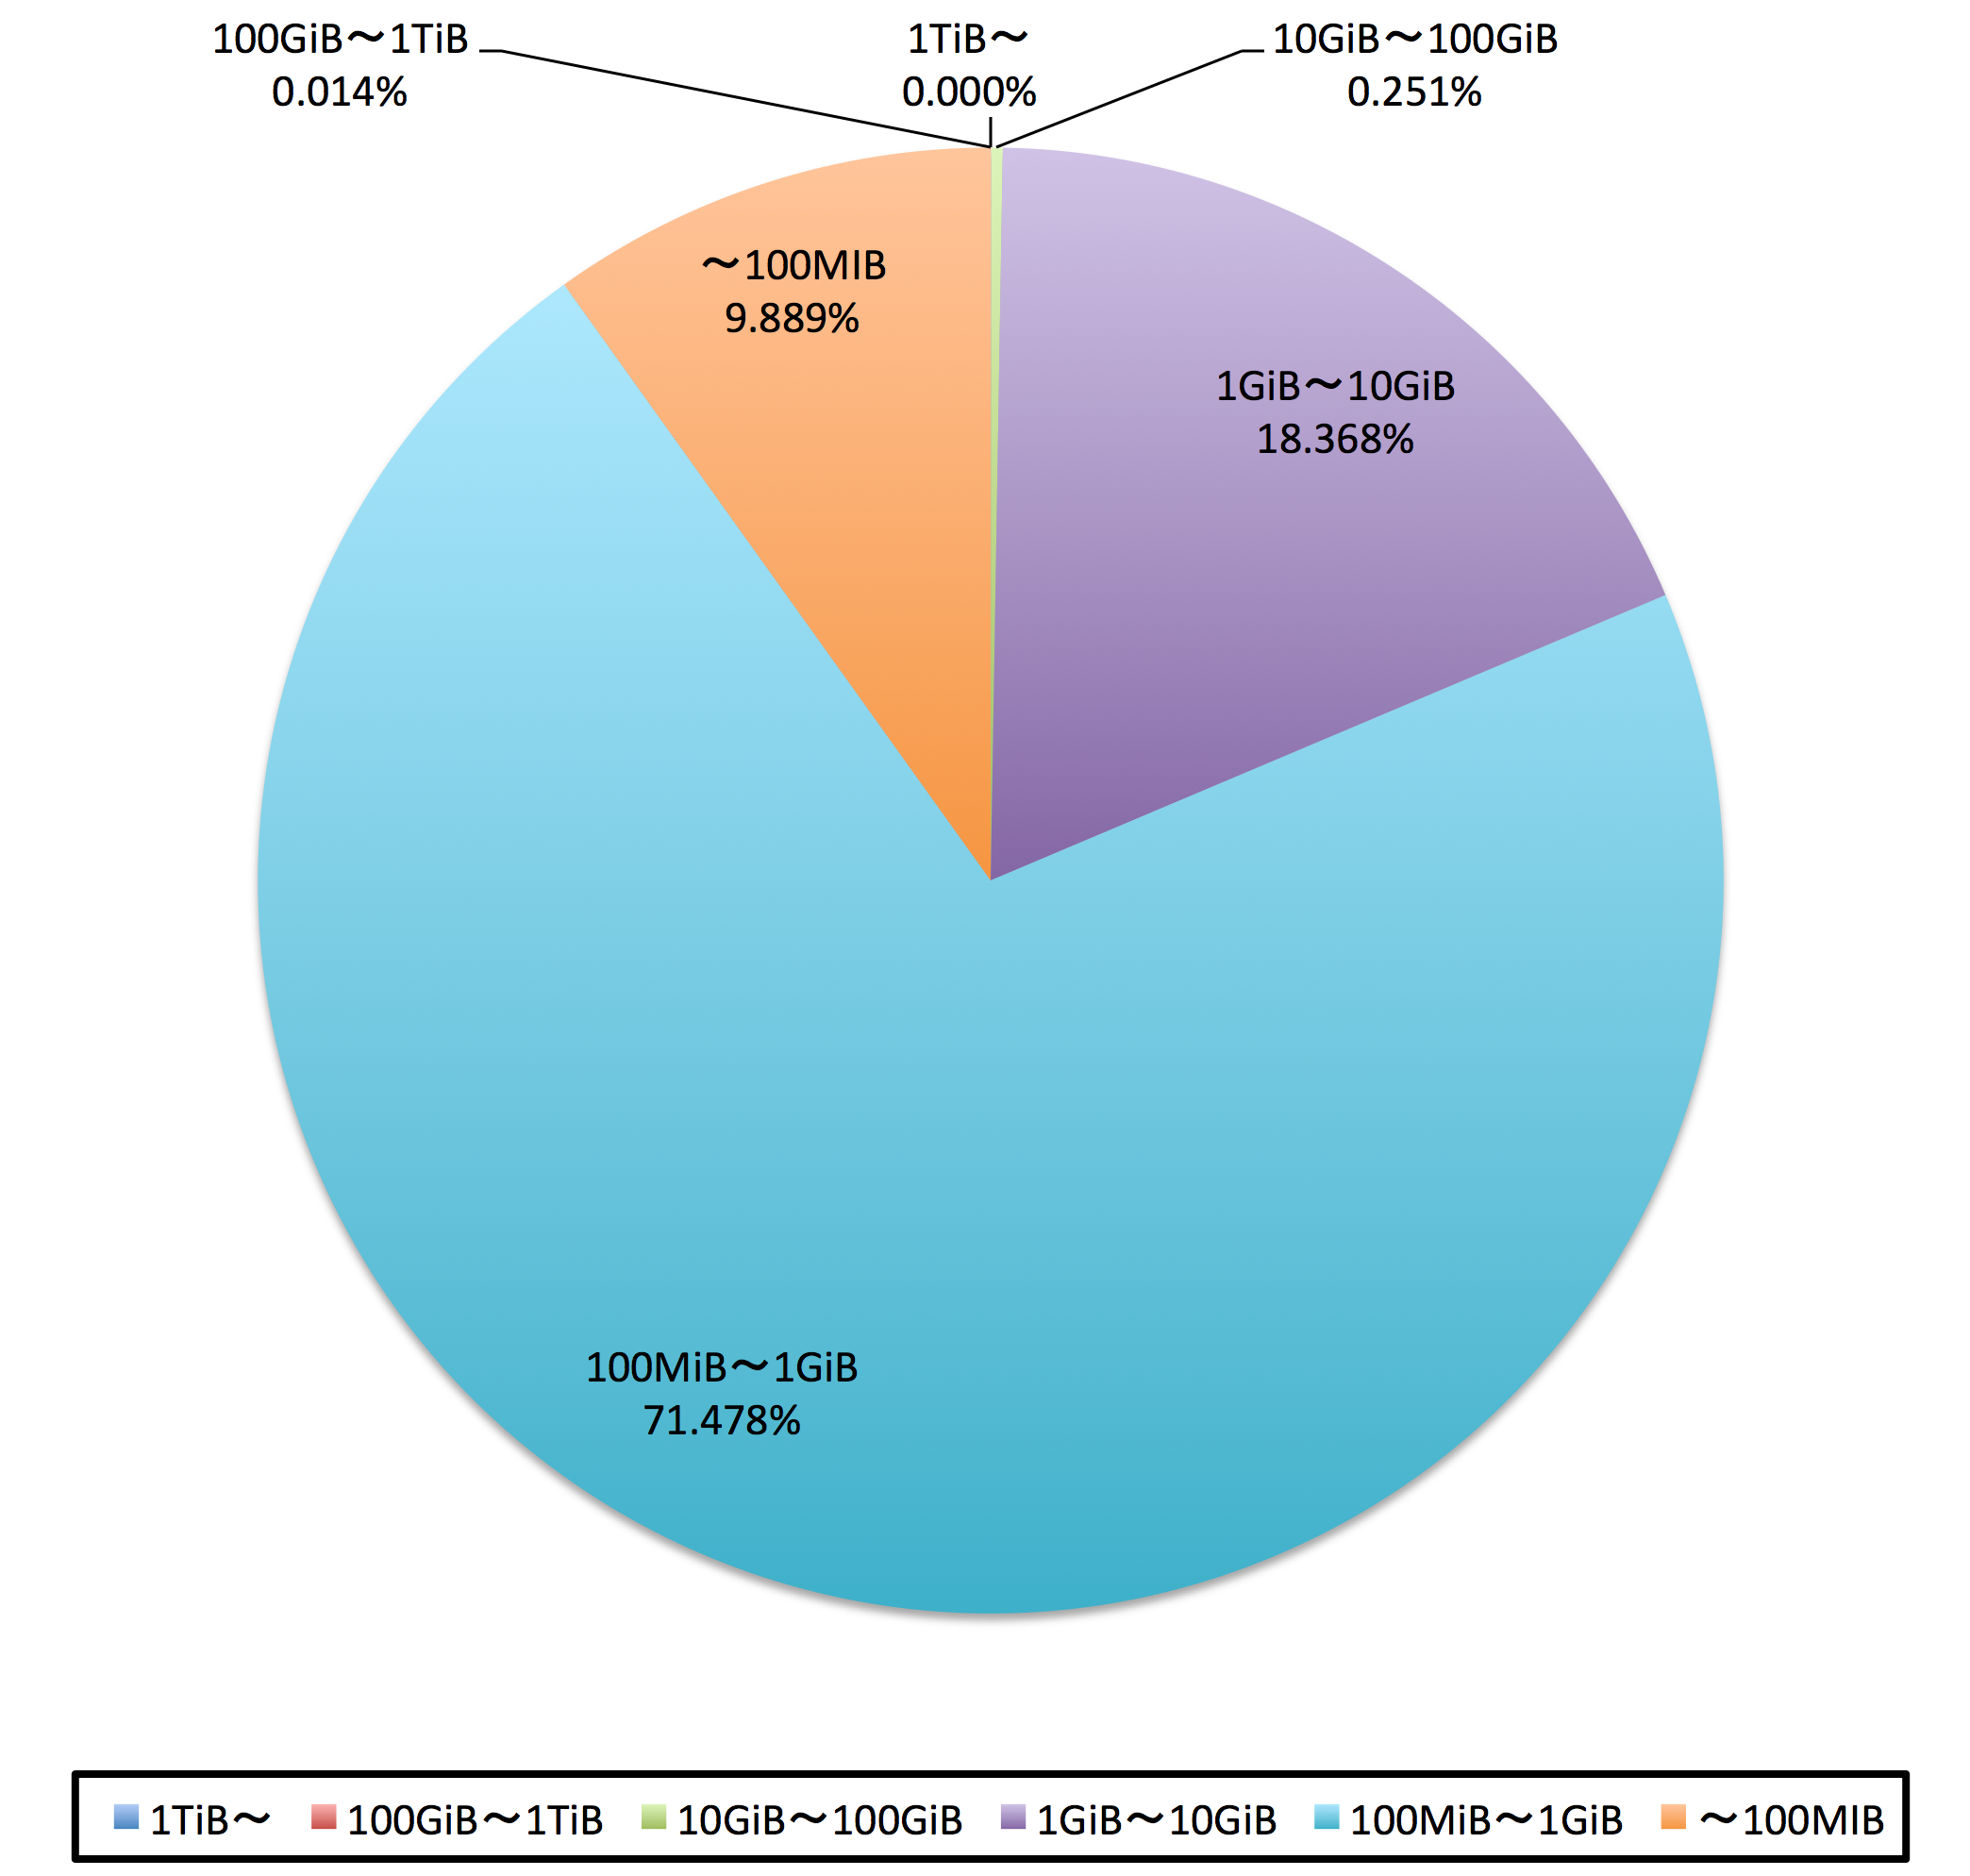
\includegraphics[clip, height=7cm, keepaspectratio] {operations/hirakawa/fig/ArchiveFileCountDistribution.png}
      \caption{File count distribution in the HPCI Archive System.}
      \locallabel{fig:ar-CountDistribution}
      \hspace{1cm}
     \end{center}
    \end{minipage}
   \end{tabular}
  \end{center}
 \end{figure}
%%%%%%%%%%%%%%%%%% Map %%%%%%%%%%%%%

\subsection{HPCI Data Analyzer West}

Another HPCI computational resource is the 88-node Linux cluster called “Data Analyzer West (DAW)”. %
 As shown in Figure \localref{fig:DAW-Construction}, the DAW's 88 computational nodes and 2 servers %
are connected via an InfiniBand network. An Intel compiler, OpenMPI, mvapich2, and GridEngine job %
scheduler are also available in the DAW environment. %
In FY2015, this cluster was made available to two HPCI research projects. %
Figure \localref{fig:DAS-JobExecutionTime} plots the monthly execution node-time occupied by %
each project and Figure \localref{fig:DAS-JobConsumptionRate} shows the job consumption rate. %
DAW was used for a total of 163\% of the allocated node-time in FY2015.

\begin{figure}[h]
 \begin{center}
  \begin{tabular}{c}

    \begin{minipage} {0.5\hsize}
     \begin{center}
      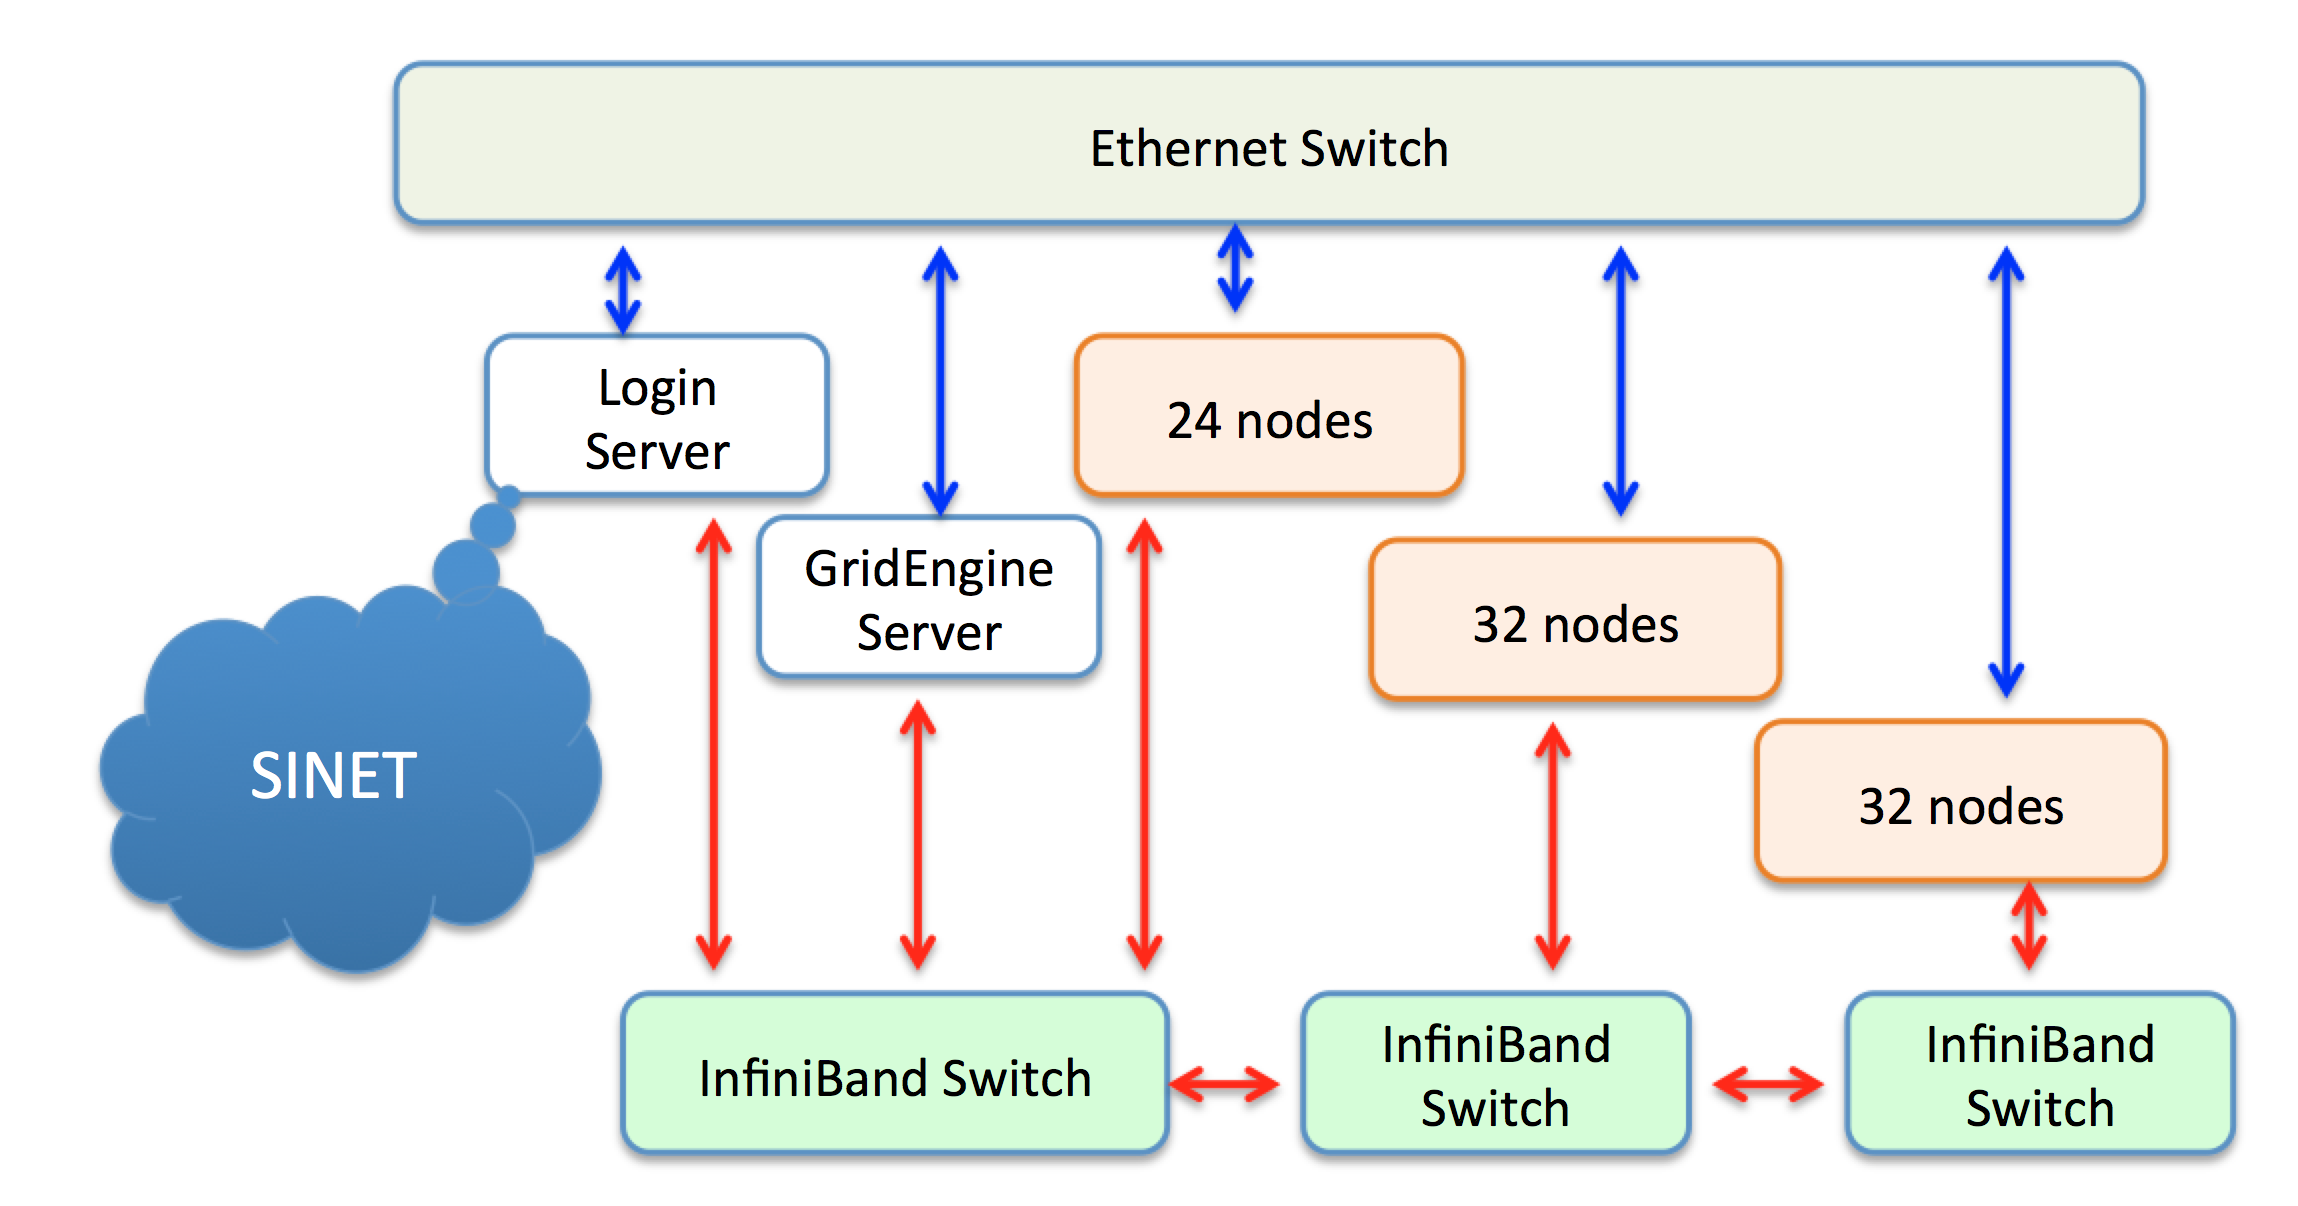
\includegraphics[clip, height=5cm, width=6.5cm] {operations/hirakawa/fig/DAS-Overview.png}
      \caption{The components of DAW.}
      \locallabel{fig:DAW-Construction}
      \hspace{1cm}
     \end{center}
    \end{minipage}

    \begin{minipage} {0.5\hsize}
     \begin{center}
      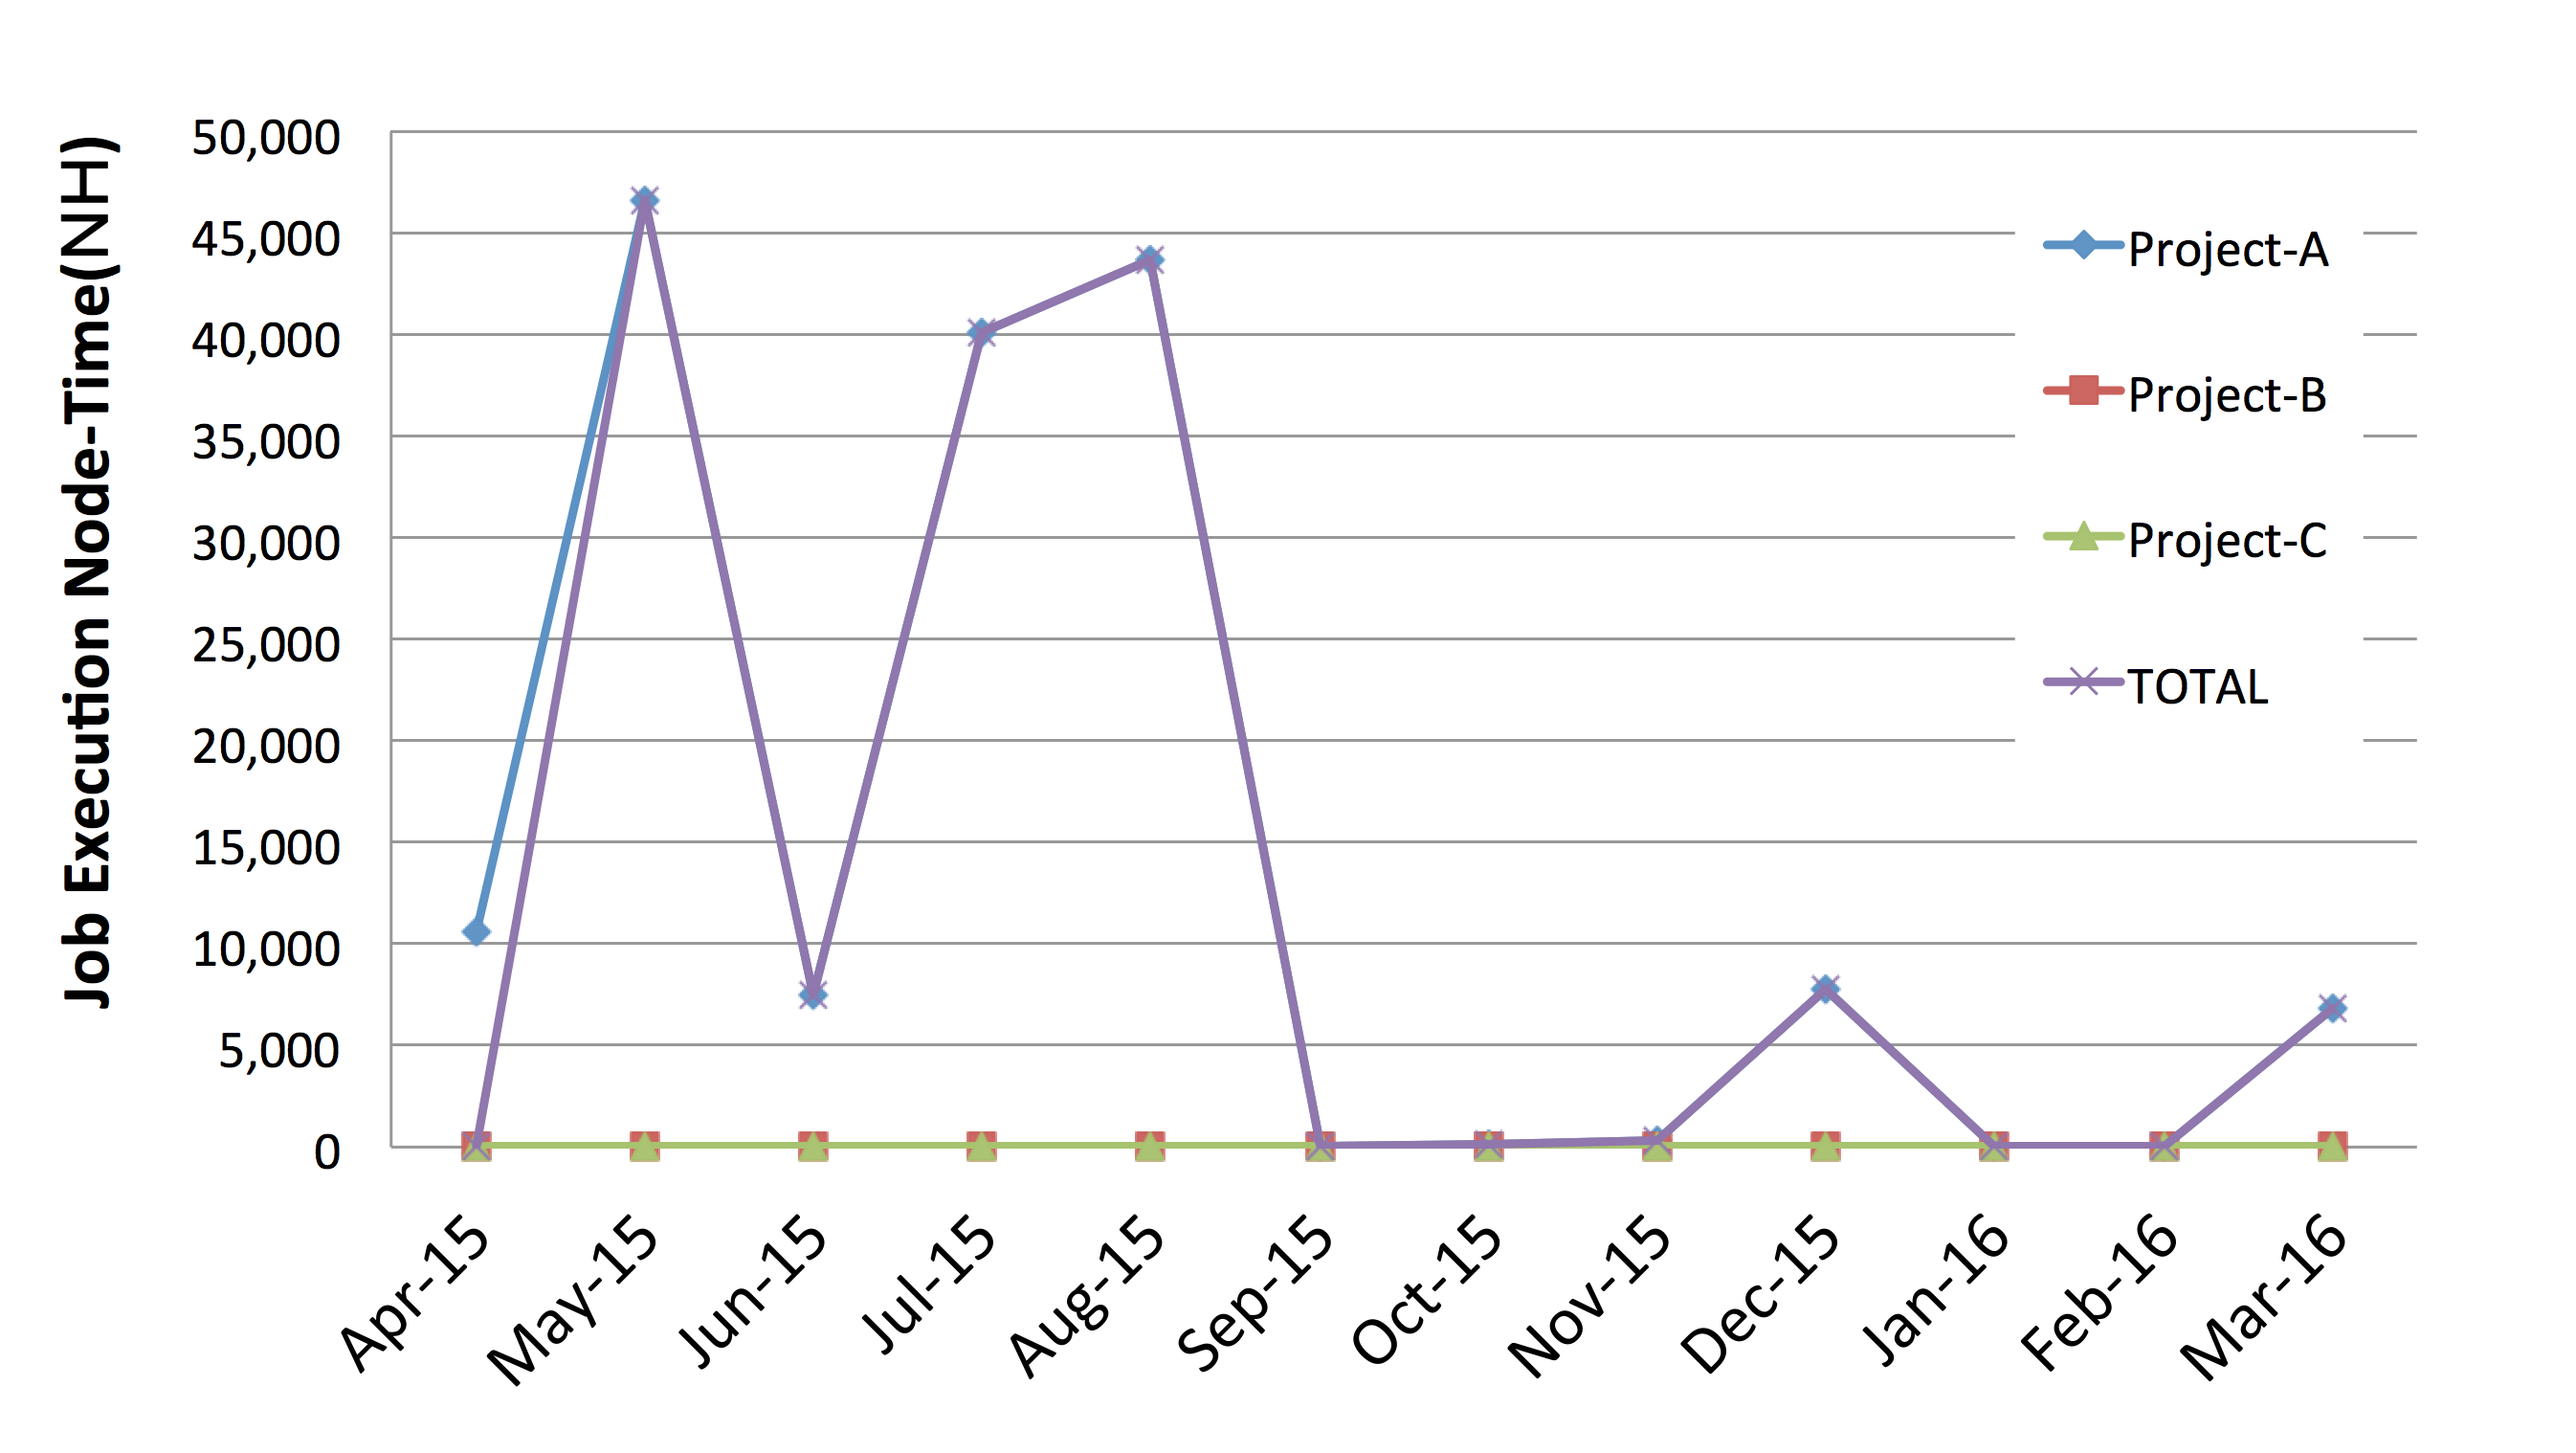
\includegraphics[clip, height=5cm, width=6.5cm] {operations/hirakawa/fig/DAS-JobExecutionTime.png}
      \caption{The monthly execution node-time for DAW.}
      \locallabel{fig:DAS-JobExecutionTime}
      \hspace{1cm}
     \end{center}
    \end{minipage}

  \end{tabular}
 \end{center}
\end{figure}

In FY2015, two HPCI research projects were chosen to use DAW, and the total allocated node-time %
was approximately 40\% of DAW capacity. It is calculated that most of the computational nodes %
remained in an idle state and that electric power was wasted. %
To reduce the power consumption of idle nodes, we introduced an automatic %
idling stop operation to the DAW computational nodes in September 2015. %
In automatic idling stop operation, idle computational nodes are shutdown automatically, %
and when jobs that need more nodes are entered in the scheduler queue, %
down state nodes are booted up to execute the job. %
Figure \localref{fig:DAS-Power} shows the DAW electric power consumption; the average monthly electric power consumption was 17472 kwh %
in normal operation and 7876 kwh in idling stop operation. As a result of the idling stop operation, we achieved an energy saving of 55\%.

\begin{figure}[h]
 \begin{center}
  \begin{tabular}{c}

    \begin{minipage} {0.5\hsize}
     \begin{center}
      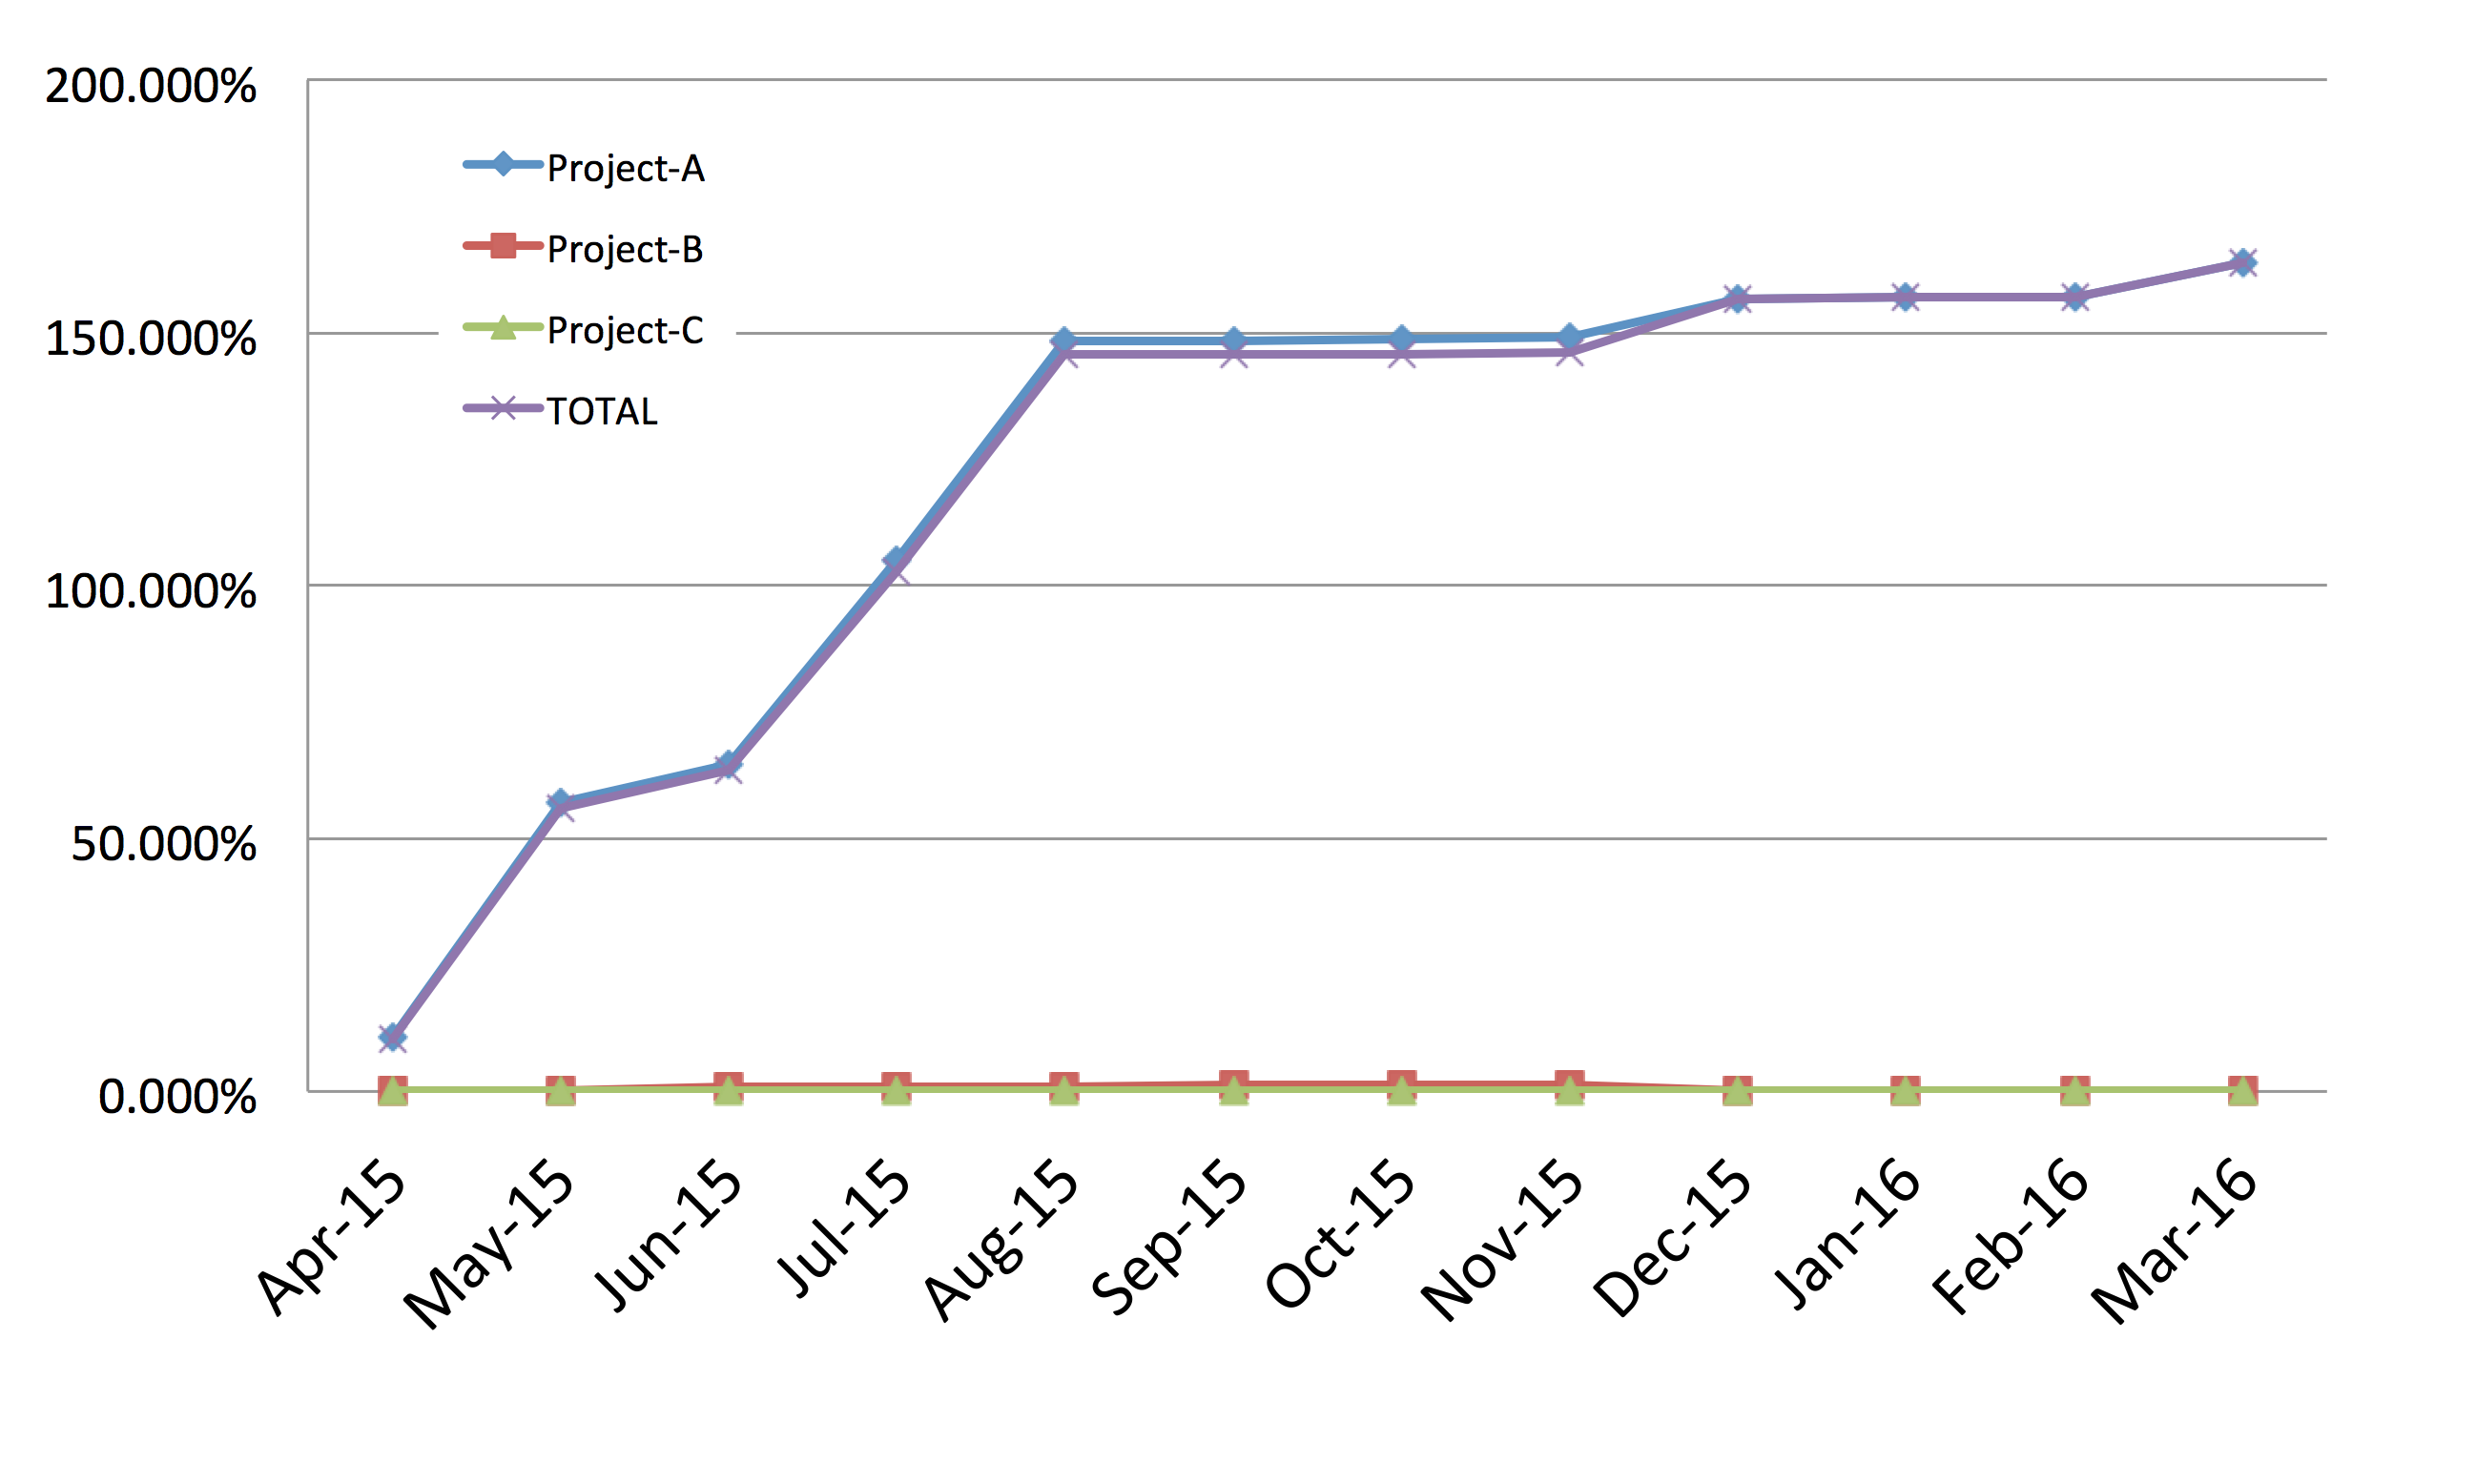
\includegraphics[clip, height=6.5cm, width=6cm] {operations/hirakawa/fig/DAS-JobConsumptionRate.png}
      \caption{DAW job consumption rate.}
      \locallabel{fig:DAS-JobConsumptionRate}
      \hspace{1cm}
     \end{center}
    \end{minipage}

    \begin{minipage} {0.5\hsize}
     \begin{center}
      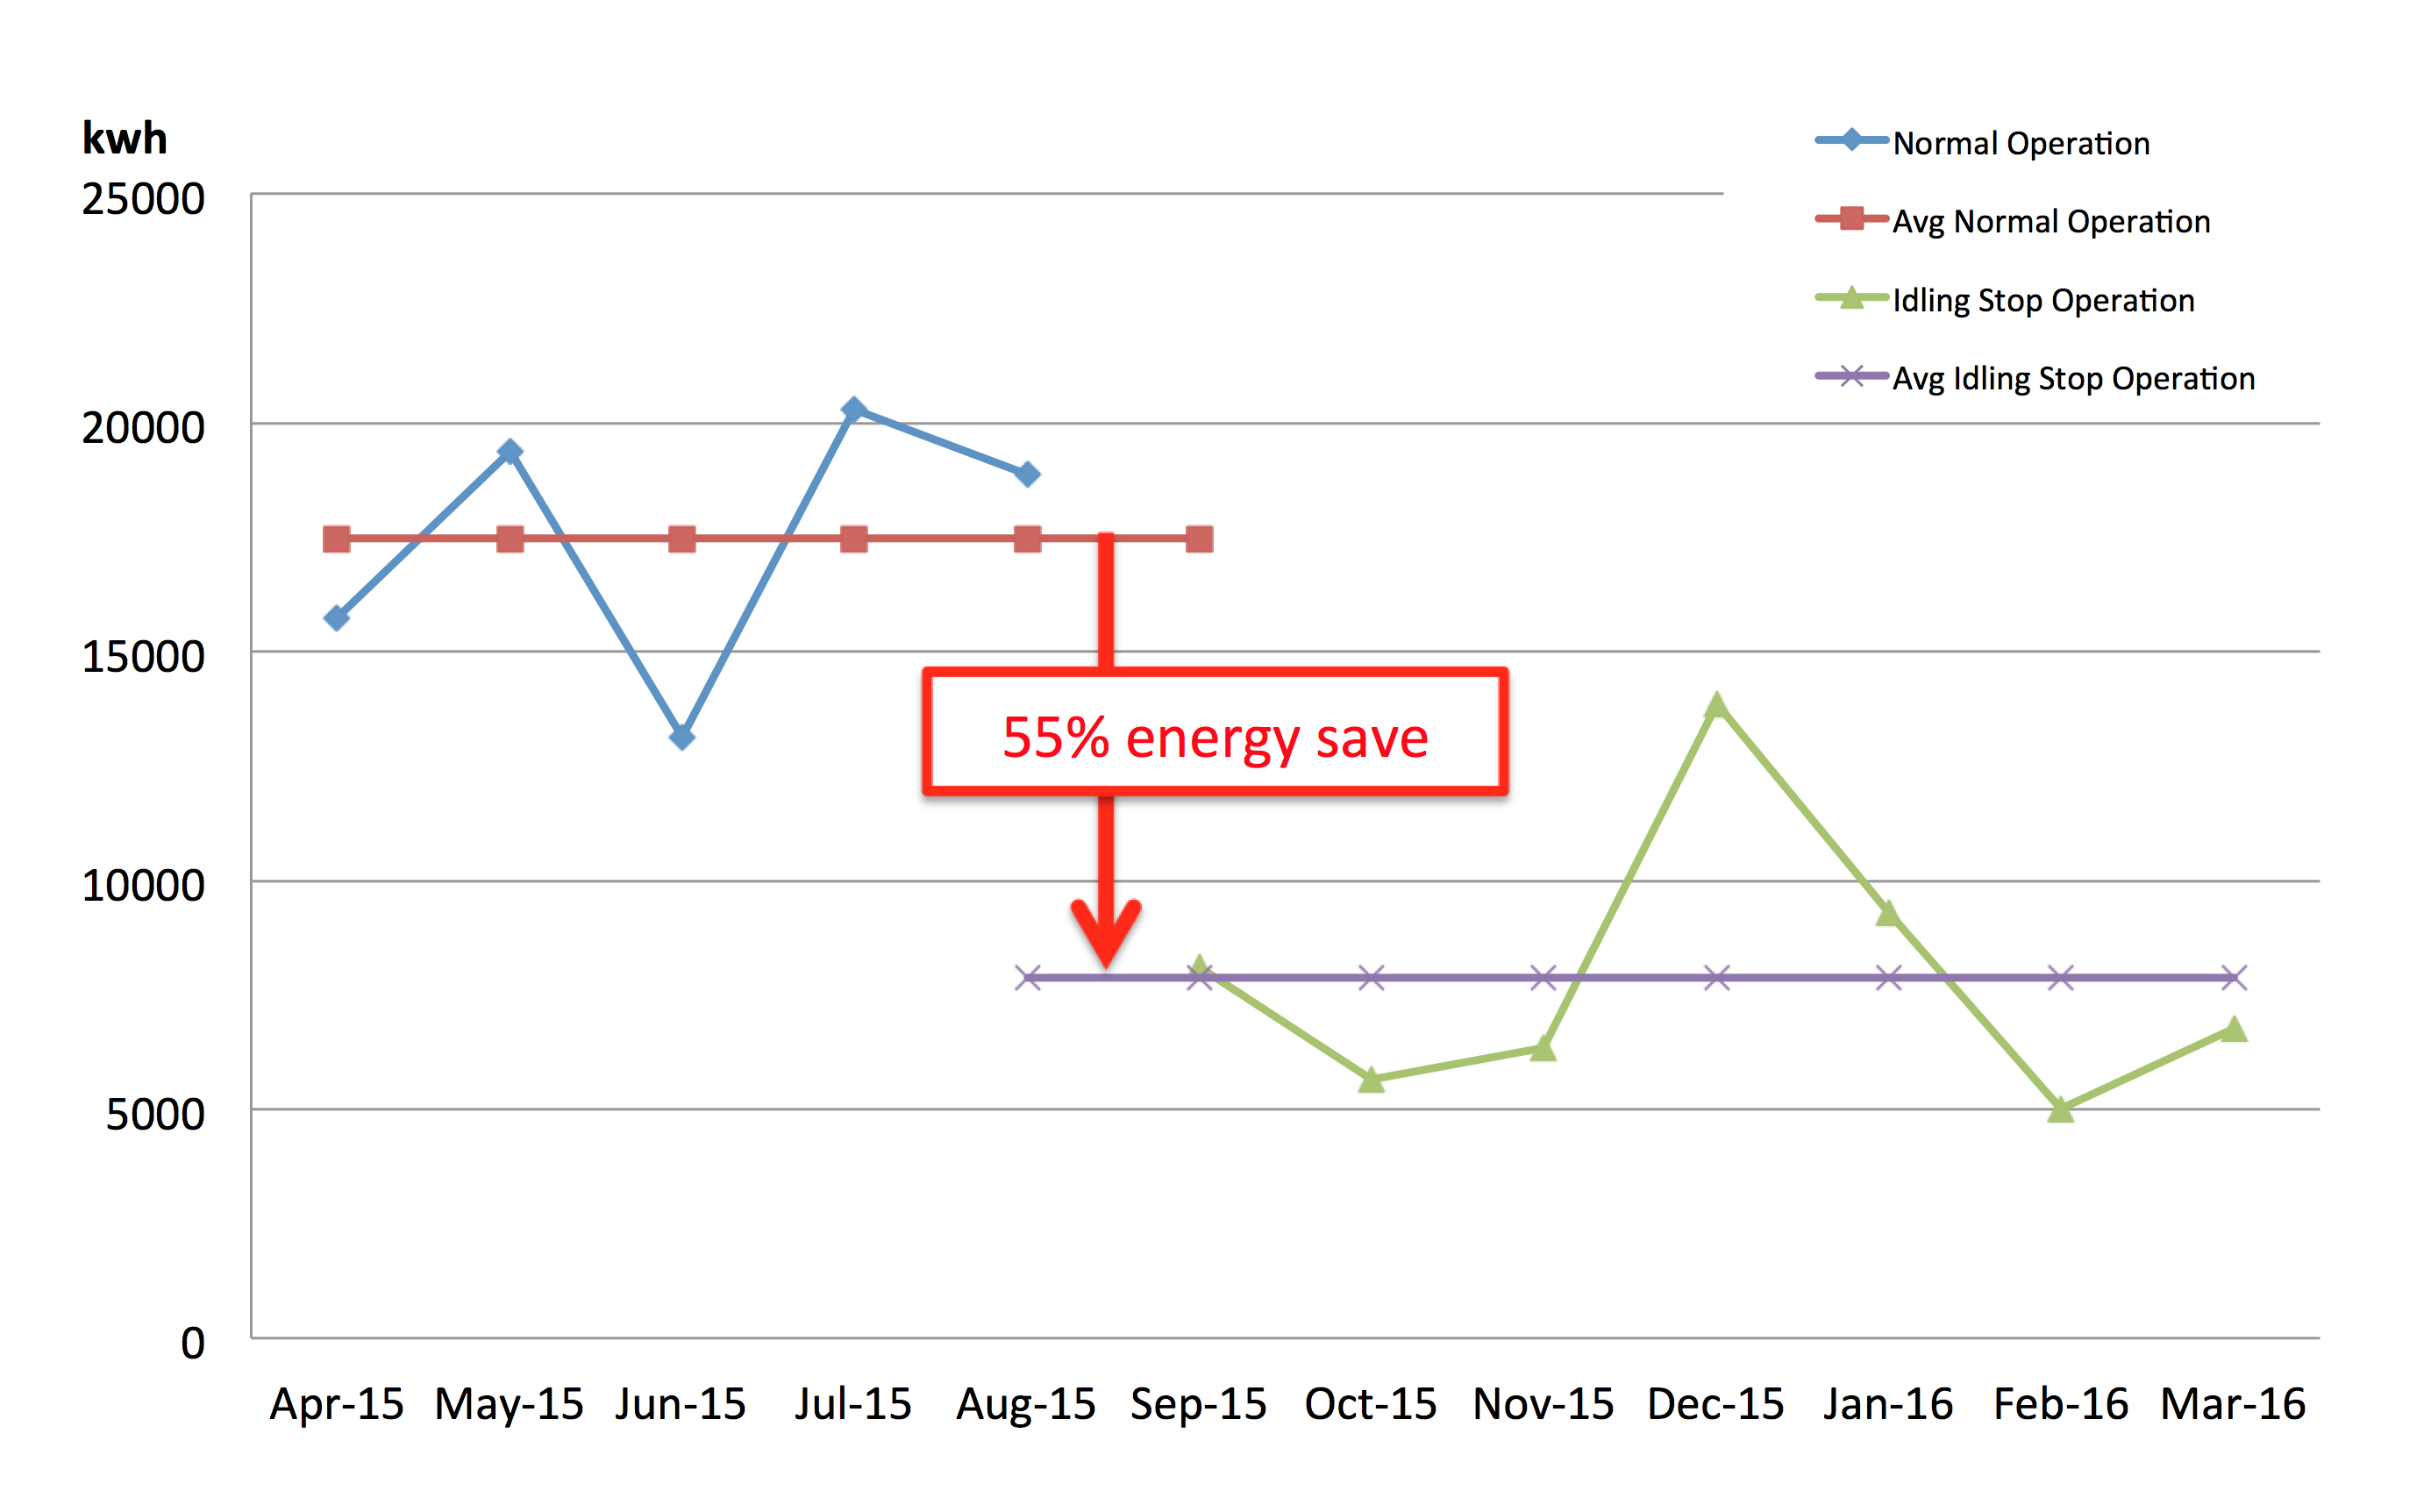
\includegraphics[clip, height=6.5cm, width=6cm] {operations/hirakawa/fig/DAS-Energy.png}
      \caption{DAW electric power consumption.}
      \locallabel{fig:DAS-Power}
      \hspace{1cm}
     \end{center}
    \end{minipage}

  \end{tabular}
 \end{center}
\end{figure}

\section{Schedule and Future Plan}

\subsection{Considerations for the second HPCI term}
HPCI is a common base infrastructure that promotes innovative computational science %
technology in Japan. It is necessary to maintain and develop this function in cooperate with %
the user communities and the HPCI system providers in the future. In the second term, %
we need to maximize our achievements, not merely by continuing the improvements and operations %
of the first term but also by accommodating the agendas that appeared in the first term and %
are newly occurring in the second term.

\subsection{Optimization of HPCI system operations}
In the coming second term, the big challenge is how to maximize our achievements and offer %
them to the public even though the computational resource structure is changing dynamically %
and the budget has tightened. We need to optimize the operations based on %
out experiences in the first term. %
In particular, compared to the first term, we need to comprehensively understand the contents of %
the inplementations within each organization to objectively see a %
comprehensive picture of an operation and evaluate it in a timely fashion, and to relay %
these findings to the operation. Therefore, in the second term, to achieve the most relevant %
operational improvements, it is necessary ro reaffirm the relationship between the HPCI %
Consortium, Japanese govement, and the HPCI system providers and to implement the PDCA cycle %
more appropriately for HPCI operations.

\subsection{Technological Planning and Coordination Affairs}
In the first term of the Technological Planning and Coordination Affairs, the HPCI cooperation service %
committee was established and operated as a place to make decisions concerning %
common services with members of the project implementing agency and the HPCI system providers. It is %
important to develop the role of this committee and to use it as a place to summarize and %
share information conductive to the PDCA cycle. For example, information %
that should be summarized, includes information concerning the amount, usage plans, and %
progress of resources, excepting the individual information of users for each project; the status of %
the achievements and problems of HPCI operation affairs; and the opinions and requests from users %
through the help desk that each project implementing agency received. For the HPCI %
cooperation service committee, to achieve the most relevant HPCI operation, it is important to %
share such information and promote cooperation with the HPCI Consortium and government for the planning %
and checking of the PDCA cycle.

%%%%%%%%%%%%%%%%%%%%%%
%\begin{figure}
%\centering
%  \includegraphics[width=1.0\textwidth,keepaspectratio,natwidth=193,natheight=40]
%  {operations/hirakawa/fig/HPCI-SS-NextGeneration.png}
%  \caption{HPCI-SS Next Generation}
%  \locallabel{fig:SS-NextGeneration}
%\end{figure}

% \subsection{Sample figure}
% Text for research Results and achievements. Journal-artcile~\cite{sample-journal}.
% Conference-paper~\cite{sample-conference}.
% Invited-talk~\cite{sample-invited}.
%
% For cross referencing, use \verb|\locallabel| and \verb|\localref| to avoid conflicting names defined by other groups. For example, a figure can be referenced as Figure~\localref{fig:sample-label1}.
%
%
% \begin{figure}
%\centering
%  \includegraphics[width=0.5\textwidth,keepaspectratio,natwidth=193,natheight=40]
%  {sample_division/sample_group/test1.png}
%  \caption{Caption for a sample figure}
%  \locallabel{fig:sample-label1}
% \end{figure}

%%% DO NOT EDIT BELOW
%
\section{Publications}

%\printbibliography[keyword=journal, heading=subbibliography, title={Journal Articles}, prefixnumbers={1-}, resetnumbers=true]
%\printbibliography[keyword=proceedings, heading=subbibliography, title={Conference Papers}, prefixnumbers={2-}, resetnumbers=true]
%\printbibliography[keyword=invited, heading=subbibliography, title={Invited Talks}, prefixnumbers={3-}, resetnumbers=true]
%\printbibliography[keyword=poster, heading=subbibliography, title={Posters and Presentations}, prefixnumbers={4-}, resetnumbers=true]
%\printbibliography[keyword=deliverable, heading=subbibliography, title={Patents and Deliverables}, prefixnumbers={5-}, resetnumbers=true]

\printbibliography[keyword=journal, heading=subbibliography, title={Journal Articles}, resetnumbers=true]
\printbibliography[keyword=proceedings, heading=subbibliography, title={Conference Papers}]
\printbibliography[keyword=invited, heading=subbibliography, title={Invited Talks}]
\printbibliography[keyword=poster, heading=subbibliography, title={Posters and Presentations}]
\printbibliography[keyword=deliverable, heading=subbibliography, title={Patents and Deliverables}]

\end{refsection}
